\documentclass[12pt]{iopart}
\usepackage[ backend=biber]{biblatex}
\addbibresource{prop.bib}
\ExecuteBibliographyOptions{sorting=none,maxbibnames=10,doi=false,isbn=false,url=false}
\usepackage{fullpage}
\usepackage[T1,T2A]{fontenc}
\usepackage[utf8]{inputenc}
\usepackage{amssymb}
\usepackage{amsthm}
\usepackage{mathrsfs}
\usepackage{bbold}
\usepackage{wesa}
\usepackage{graphicx}
\usepackage{verbatim}
\usepackage{iopams}
\usepackage{setstack}

\theoremstyle{plain}
\newtheorem{thm}{Theorem}
\newtheorem{lemma}[thm]{Lemma}
\newtheorem{cor}[thm]{Corollary}
\theoremstyle{definition}
\newtheorem{definition}[thm]{Definition}
\newtheorem{example}[thm]{Example}

\newcommand{\Hilb}{\mathcal{H}}
\newcommand{\events}{\ensuremath{\mathcal{E}}}
\newcommand{\qevents}{\ensuremath{\mathcal{E}}}
\newcommand{\pmeas}{\ensuremath{\mu}}
\newcommand{\imposs}{{\mbox{\wesa{impossible}}}}
\newcommand{\likely}{{\mbox{\wesa{likely}}}}
\newcommand{\unlikely}{{\mbox{\wesa{unlikely}}}}
\newcommand{\necess}{{\mbox{\wesa{certain}}}}
\newcommand{\unknown}{{\mbox{\wesa{unknown}}}}
\newcommand{\midd}{{\mbox{\wesa{middle}}}}
\newcommand{\ket}[1]{{\left\vert{#1}\right\rangle}}
\newcommand{\fket}[1]{{|#1\rangle}}
\newcommand{\fproj}[1]{|#1\rangle\langle #1|}
\newcommand{\op}[2]{\ensuremath{\left\vert{#1}\middle\rangle\middle\langle{#2}\right\vert}}
\newcommand{\proj}[1]{\op{#1}{#1}}
\newcommand{\ps}{\texttt{+}}
\newcommand{\minus}{\texttt{-}}
\newcommand{\ip}[2]{\ensuremath{\left\langle{#1}\middle\vert{#2}\right\rangle}}

\usepackage{color}
\usepackage[usenames,dvipsnames]{xcolor}
\newcommand{\amr}[1]{\fbox{\begin{minipage}{0.9\textwidth}\color{green}{Amr says: #1}\end{minipage}}}
\newcommand{\yutsung}[1]{\fbox{\begin{minipage}{0.9\textwidth}\color{purple}{Yu-Tsung says: #1}\end{minipage}}}
\newcommand{\set}[2]{\ensuremath{\left\{ {#1}~\middle|~{#2}\right\} }}
\def\C{{\mathbb{C}}}

\begin{document}
\title{Measurement and Probability in Fuzzy Quantum
Theories}

\author{Andrew J Hanson$^{1}$, Gerardo Ortiz$^{2}$,
Amr Sabry$^{1}$ and Yu-Tsung Tai$^{3,1}$}
\address{$^{1}$ School of Informatics and Computing, Indiana
University, Bloomington, IN 47405, USA}
\address{$^{2}$ Department of Physics, Indiana University, Bloomington, IN
47405, USA}
\address{$^{3}$ Department of Mathematics, Indiana University, Bloomington,
IN 47405, USA}
\ead{ortizg@indiana.edu}
\begin{abstract}
\today
\end{abstract}
\pacs{03.65.-w, 03.65.Ta, 02.40.Dr, 02.50.Cw, 02.50.Le}
\noindent{\it Keywords\/}: {Finite precision measurement, the Born rule, Gleason's theorem, interval-valued
probability, discrete quantum theory}

\submitto{\jpa}

%%%%%%%%%%%%%%%%%%%%%%%%%%%%%%%%%%%%%%%%%%%%%%%%%%%%%%%%%%%%%%%%%%%%%%%%%%%%%%
\section{Introduction}

Textbook quantum mechanics asserts that, given a quantum spin system
described by the wave function
$\ket{\psi}=\frac{\sqrt{\pi}}{2}\fket{\ps\frac{1}{2}}+\frac{\sqrt{4-\pi}}{2}\fket{\minus\frac{1}{2}}$
and given the observable
$S_z =
\frac{\hbar}{2}(\fproj{\ps\frac{1}{2}}-\fproj{\minus\frac{1}{2}})$,
then the probability of observing the eigenvalue $\ps\frac{\hbar}{2}$
(with post-measurement state $\fket{\ps\frac{1}{2}}$) is
$\frac{\pi}{4}$ and the probability of observing the eigenvalue
$\minus\frac{\hbar}{2}$ (with post-measurement state
$\fket{\minus\frac{1}{2}}$) is $1-\frac{\pi}{4}$. According to the
frequency interpretation of probability, the above assertion implies
that when performing a very large number of experiments on quantum
systems described by wave function $\ket{\psi}$, a fraction
$\frac{\pi}{4}$ of the experiments will result in the observation
$\ps\frac{\hbar}{2}$ and the remaining fraction $1-\frac{\pi}{4}$ will
result in the observation $\minus\frac{\hbar}{2}$.

In reality, i.e., in an actual experiment, simulation, or computation,
bounded by space, time, and energy resources, the situation is much
fuzzier: (i) we cannot \emph{exactly} prepare the state $\ket{\psi}$;
(ii) we cannot build a measurement apparatus corresponding
\emph{exactly} to observable $S_z$; and (iii) we cannot prepare
\emph{exact} replicas of any state. In other words, we can only
perform a limited number of experiments on quantum systems closely
related to wave function $\ket{\psi}$ and using an apparatus that
closely approximates observable $S_z$. Given any fixed resources,
these experiments will \emph{not} result in the \emph{exact} fraction
$\frac{\pi}{4}$ of observations $\ps\frac{\hbar}{2}$ and
$1-\frac{\pi}{4}$ of observations $\minus\frac{\hbar}{2}$. In fact,
these experiments can be viewed as a method (algorithm) to calculate
the value $\pi$ and it is known that the state of the art algorithms
for computing the $n$th binary digit of~$\pi$ require on the order of
$O\left(n\log^{O\left(1\right)}\left(n\right)\right)$
operations~\cite{journals/moc/BaileyBP97}. In other words, calculating
the $n$th digit of $\pi$ appears to require more and more physical
resources as~$n$ gets larger.

All of this is well-known and holds in both the classical and quantum
worlds. In the classical world, these observations are believed to be
well-understood approximations to an idealized independent reality
that can continuously approached with more and more resources. The
question in the quantum world is more subtle; it is not evident at all
that this resource-aware perspective does not alter the very
foundations of quantum mechanics. Indeed taking such resource bounds
into consideration is what founded computer science as a discipline
and has become crucial for understanding the very nature of
computation. Following Feynman~\cite{Feynman1982Simulating},
Landauer~\cite{Landauer1996188}, and others, one might argue that this
resource-bounded perspective is also crucial for understanding the
very nature of physical processes.

In previous work, we analyzed the wave function description of quantum
systems from a resource-bounded perspective. Technically, instead of
postulating that quantum states are rays in a Hilbert space, i.e., we
instead used special finite fields whose size reflected the available
resources. \ldots

\newpage

This is a \emph{theoretical} investigation of \emph{experimental}
physics using \emph{computational} methods. All experiments and computations
are processes bounded in space, time, energy, and other resources~\cite{Jaeger2007,Piccinini2015}.
Yet, for centuries, the mathematical formalization of such processes
has been founded on the infinitely precise real or complex numbers~\cite{Ziegler2007,weihrauch2012computable,blum2012complexity}.
Our purpose here is to exploit the consequences of replacing infinitely-specified
quantum probabilities by finite number of intervals used in interval-valued
probability measures~(IVPM); in particular, we show that a quantum
IVPM may not be induced by a infinitely-precise state, but it might
be more and more likely to be identified to a particular state when
the measurement resources increase.

Indeed, almost every description of quantum mechanics, quantum computation,
or quantum experiments refers to entities such as $\rme$, $\pi$,
$\sqrt{2}$, etc (see, e.g., \cite{Redhead1987-REDINA,544199,Mermin2007}).
From a computational perspective, such numbers do not exist in their
entirety ``for free~\cite{Kent1999,CliftonKent2000}.'' For example,
the state of the art algorithms for computing the $n$th binary digit
of~$\pi$ require on the order of $O\left(n\log^{O\left(1\right)}\left(n\right)\right)$
operations~\cite{journals/moc/BaileyBP97}. In other words, simply
referring to the $n$th digit of $\pi$ requires more and more resources
as $n$ gets larger. Taking such resource bounds into consideration
is what founded computer science as a discipline and is crucial for
understanding the very nature of computation and, following Feynman~\cite{Feynman1982Simulating},
Landauer~\cite{Landauer1996188}, and others, for understanding the
very nature of physical processes.

We have been revisiting quantum mechanics, quantum information, and
quantum computation from this resource-aware perspective. Our initial
results in that domain showed how subtle the issues can be~\cite{usat,geometry2013,DQT2014}:
a straightforward replacement of the complex numbers by a finite field
yields a variant of quantum mechanics in which computationally hard
problems like UNIQUE-SAT (which decides whether a given Boolean formula
is unsatisfiable or has exactly one satisfying assignment~\cite{Valiant198685,Papadimitriou1993,AroraBarak2009})
can be deterministically solved in constant time. To eliminate such
unrealistic theories requires delicate analysis of the structure of
the Hilbert space, the process of observation, and the notion of probability
teasing apart their reliance on the infinitely precise real numbers~\cite{geometry2013,DQT2014}. 

In this paper, we shift focus from the infinitely-specified but not
directly observable quantum states, to observable measurable properties
of quantum systems and their probabilities. Furthermore, we insist
that our theories of measurement and probability only refer to finitely
communicable evidence within feasible computational bounds. It follows
that states, observations, and probabilities all become ``fuzzy'',
i.e., specified by intervals of confidence that can only increase
in precision if the available resources increase proportionally. Our
notion of ``fuzzy quantum mechanics'' is related to existing work~\cite{GranikCaulfield1996,Pykacz2013,SNL2009,Gudder2005,aerts1993physical}
but, as will be explained in more detail, is distinguished by its
unique computational character.

We will begin by reviewing existing work that recasts classical probability
spaces in a resource-aware setting and move to aim at recasting quantum
probability and quantum measurement. In particular, we develop a measurement
framework based on quantum IVPM. Surprisingly, we found a quantum
IVPM which can not be induced by a state, while Shapley proved a classical
convex IVPM can always be induced by a classical ``state''~\cite{Shapley1971,Grabisch2016},
and Gleason proved a infinitely-specified quantum probabilities measure
can always be induced by a quantum state~\cite{gleason1957,Redhead1987-REDINA,peres1995quantum}.
Nevertheless, a quantum IVPM could still correspond to many possible
states if it is broken into pieces. Our examples also suggest that
a quantum IVPM could be more and more likely induced by a state while
the intervals become sharper, i.e., the measurement resources increase.

Since Gleason's theorem supports the idea of von Neumann to define
a state as a density matrix~\cite{Varadarajan2008}, a density matrix
might not be a adequate imprecise quantum state. Instead, a imprecise
quantum state might be more like an interactive system suggested by
Quantum Bayesianism or QBism~\cite{FuchsSchack2013,FuchsMerminSchack2014,VonBaeyer2016},
which would interact differently with different clients. Furthermore,
the validity the fundamental theorems of quantum mechanics followed
up by Gleason's theorem, such as Bell~\cite{Bell1964,Redhead1987-REDINA,peres1995quantum,Jaeger2007}
and Kochen-Specker~\cite{kochenspecker1967,Redhead1987-REDINA,peres1995quantum,Jaeger2007},
might need to be reassessed based on our imprecise measurement. Our
research then might provide a new insight to the old debate among
Meyer, Mermin, and others about whether finite precision measurement
would nullify the Kochen-Specker theorem or not~\cite{PhysRevLett.83.3751,Mermin1999,BarrettKent2004}.

%%%%%%%%%%%%%%%%%%%%%%%%%%%%%%%%%%%%%%%%%%%%%%%%%%%%%%%%%%%%%%%%%%%%%%%%%%%%%%
\section{Classical Probability}

A \emph{probability space} specifies the necessary conditions for
reasoning coherently about collections of uncertain
events~\cite{Kolmogorov1950,Shafer1976,Griffiths2003,Swart2013}.  We
review the conventional presentation of probability spaces and then
discuss the computational resources needed to estimate probabilities.

%%%
\subsection{Classical Probability Spaces}

The conventional definition of a probability space builds upon the
field of real numbers. In more detail, a probability space consists
of a \emph{sample space} $\Omega$, a space of \emph{events}~$\events$,
and a \emph{probability measure}~$\pmeas$ mapping events in $\events$
to the real interval $[0,1]$. We will only consider \emph{finite}
sets of events and restrict our attention to non-empty finite sets
$\Omega$ as the sample space. The space of events $\events$ includes
every possible subset of $\Omega$: it is the powerset~$2^{\Omega}=\set{E}{E\subseteq\Omega}$.
For future reference, we emphasize that events are the primary notion
of interest and that the sample space is a convenient artifact that
allows us to treat events as sets obeying the laws of Boolean algebra~\cite{Boole1948,Redhead1987-REDINA,Griffiths2003}.

\begin{definition}[Probability Measure]\label{def:ClassicalProbabilitySpace}
  Given the set of events $\events$, a \emph{probability measure} is a
  function $\pmeas:\events\rightarrow[0,1]$ such that:
\begin{itemize}
\item $\pmeas(\emptyset)=0$,
\item $\pmeas(\Omega)=1$, 
\item for every event $E$,
  $\pmeas\left(\Omega\backslash E\right)=1-\pmeas\left(E\right)$ where
  $\Omega\backslash E$ is the complement event of $E$, and
\item for every collection $\left\{ E_{i}\right\} _{i=1}^{N}$ of
  pairwise disjoint events,
  $\pmeas\left(\bigcup_{i=1}^{N}E_{i}\right)=\sum_{i=1}^{N}\pmeas(E_{i})$.
\end{itemize}
\end{definition}
\noindent There is some redundancy in the definition that will be useful when
moving to quantum probability spaces. 

\begin{example}[Two-coins experiment]\label{ex1} Consider an
  experiment that tosses two coins. We have four possible outcomes
  that constitute the sample space $\Omega=\{HH,HT,TH,TT\}$. There are
  16 total events including the event $\{HH,HT\}$ that the first coin
  lands heads up, the event $\{HT,TH\}$ that the two coins land on
  opposite sides, and the event $\{HT,TH,TT\}$ that at least one coin
  lands tails up. Here is a possible probability measure for these
  events:
\begin{equation}
\begin{array}{c@{\qquad\qquad}c}
\begin{array}{rcl}
\pmeas(\emptyset) & = & 0\\
\pmeas(\{HH\}) & = & \frac{1}{3}\\
\pmeas(\{HT\}) & = & 0\\
\pmeas(\{TH\}) & = & \frac{2}{3}\\
\pmeas(\{TT\}) & = & 0\\
\pmeas(\{HH,HT\}) & = & \frac{1}{3}\\
\pmeas(\{HH,TH\}) & = & 1\\
\pmeas(\{HH,TT\}) & = & \frac{1}{3}
\end{array} & \begin{array}{rcl}
\pmeas(\{HT,TH\}) & = & \frac{2}{3}\\
\pmeas(\{HT,TT\}) & = & 0\\
\pmeas(\{TH,TT\}) & = & \frac{2}{3}\\
\pmeas(\{HH,HT,TH\}) & = & 1\\
\pmeas(\{HH,HT,TT\}) & = & \frac{1}{3}\\
\pmeas(\{HH,TH,TT\}) & = & 1\\
\pmeas(\{HT,TH,TT\}) & = & \frac{2}{3}\\
\pmeas(\{HH,HT,TH,TT\}) & = & 1
\end{array}\end{array}
\end{equation}
\end{example}

\noindent It is useful to think that this probability measure is
completely determined by the ``reality'' of the two coins in question
and their characteristics, in the sense that each pair of coins
induces a measure, and each measure must correspond to some pair of
coins. The measure above would be induced by two particular coins such
that the first coin is twice as likely to land tails up than heads up
and the second coin is double-headed. 

%%%%%
\subsection{Measuring Probabilities: Buffon's Needle Problem\label{subsec:Measuring-Probabilities:-Buffon}}

In a strict computational or experimental setting, one should question
the reliance of the definition of probability space on the uncountable
and uncomputable real
interval~$[0,1]$~\cite{Turing_1937,Ziegler2007,weihrauch2012computable}.
This interval includes numbers like $0.h_{1}h_{2}h_{3}\ldots$ where
$h_{i}$ is 1 or 0 depending on whether Turing machine
$\mathit{TM}_{i}$ halts or not. Such numbers cannot be computed. This
interval also includes numbers like $\pi / 4$ which can only be
computed with increasingly large resources as the precision
increases. Therefore, in a resource-aware computational or
experimental setting, it is more appropriate to consider probability
measures that map events to a set of elements computable with a fixed
set of resources. We expand on this observation in the next section
and then recall its formalization using interval-valued probability
measures~\cite{Weichselberger2000,JamisonLodwick2004}.
 
In the previous example, we assumed the probability~$\pmeas(E)$ of
each event~$E$ is known a priori. In reality, although each event is
assumed to have a probability, the exact value of $\pmeas(E)$ may not
be known. According to the \emph{frequency interpretation of
  probability} (which we will revisit when moving to the quantum
case)~\cite{Venn1876,Hajek2012}, 
to determine the probability of an event, we run $M$
independent trials which gives us an approximation of the (assumed)
``true'' or ``real'' probability. Let $x_{i}$ be 1 or 0 depending on
whether the event~$E$ occurs in the $i$-th trial or not, then
$\pmeas(E)$ could be approximated to given accuracy~$\epsilon>0$ by
the relative frequency~$\sum_{i=1}^{M}x_{i} / M$ with the
probability converging to one as $M$ goes to infinity, i.e.,
\begin{equation}
\forall\epsilon>0,\lim_{M\rightarrow\infty}\pmeas\left(\left|\pmeas(E)-\frac{1}{M}\sum_{i=1}^{M} x_{i}\right|<\epsilon\right)=1\textrm{ .}
\end{equation}
This fact is called the law of large numbers~\cite{Bernoulli2006,Kolmogorov1950,Uspensky1937,Shafer1976,544199}.

Let's look at a concrete example. Suppose we drop a needle of length
$\ell$ onto a floor made of equally spaced parallel lines a distance
$h$ apart, where $\ell<h$. It is a known fact that the probability of
the needle crossing a line is
$2\ell/\left(\pi h\right)$~\cite{Buffon1777,DeMorgan1872,Hall1873,Uspensky1937}.
Consider an experimental setup consisting of a collection of $M$
identical needles of length $\ell$. We throw the $M$ needles one
needle at a time, and observe the number $M_c$ of needles that cross a
line, thus estimating the probability of a needle crossing a line to
be $M_c/M$. In an actual experiment with $500$ needles and the
ratio $\ell/h=0.75$~\cite{Hall1873}, it was found that $236$
crossed a line so the relative frequency is $0.472$ whereas the
idealized mathematical probability is $0.4774\ldots$.  In a larger
experiment with $5000$ needles and the ratio
$\ell/h=0.8$~\cite{Uspensky1937}, the relative frequency was
calculated to be $0.5064$ whereas the idealized mathematical
probability is $0.5092\ldots$. We see that the observed probability
approaches $2\ell/\left(\pi h\right)$ but only if \emph{larger and larger
  resources} are expended. These resource considerations suggest that
it is possible to replace the real interval $[0,1]$ with rational
numbers up to a certain precision related to the particular experiment
in question. There is clearly a connection between the number of
needles and the achievable precision: in the hypothetical experiment
with 3 needles, it is not sensible to retain 100 digits in the
expansion of $2\ell/\left(\pi h\right)$.

There is another more subtle assumption of unbounded computational
power in the experiment. We are assuming that we can always determine
with certainty whether a needle is crossing a line. But ``lines'' on
the the floor have thickness, their distance apart is not exactly $h$,
and the needles' lengths are not all absolutely equal to $\ell$.
These perturbations make the events ``fuzzy.'' Thus, in an experiment
with limited resources, it is not possible to talk about the idealized
event that exactly $M_c$ needles cross lines as this would require the
most expensive needles built to the most precise accuracy, laser
precision for drawing lines on the floor, and the most powerful
microscopes to determine if a needle does cross a line. Instead we
might talk about the event that $M_c-\delta$ needles evidently cross
lines and $M_c+\delta'$ needles plausibly cross lines where $\delta$ and
$\delta'$ are resource-dependent approximations. This fuzzy notion of
events leads to probabilities being only calculable within intervals
of confidence reflecting the certainty of events and their
plausibility. This is indeed consistent with published experiments: in
an experiment with $3204$ needles and the ratio
$\ell/h=0.6$~\cite{DeMorgan1872}, $1213$ needles clearly
crossed a line and $11$ needles were close enough to plausibly be
considered as crossing the line: we would express the probability in
this case as the interval
$\left[\frac{1213}{3204},\frac{1224}{3204}\right]$ expressing that we
are certain that the event has probability at least
$\frac{1213}{3204}$ but it is possible that it would have probability
$\frac{1224}{3204}$.

Another way to re-express the above observations is that the calculus
of probabilities requires all probabilities to be \emph{coherent}
(e.g., the probability of the union of two disjoint events is the sum
of their probabilities). But given limited resources, the calculation
of a probability measure can only be approximate and hence the
probabilities cannot be absolutely guaranteed to be coherent in the
ideal sense. 

%%%%%
\subsection{Classical Interval-Valued Probability Measures}

As motivated above, an event $E_{1}$ may have an interval of probability
$[l_{1},r_{1}]$. Assume that another disjoint event $E_{2}$ has
an interval of probability $[l_{2},r_{2}]$, what is the interval
of probability for the event $E_{1}\cup E_{2}$? The answer is somewhat
subtle: although it is possible to use the sum of the intervals $[l_{1}+l_{2},r_{1}+r_{2}]$
as the combined probability, one can find a much tighter interval
if information \emph{against} the event (i.e., information about the
complement event) is also taken into consideration. Formally, for
a general event $E$ with probability $[l,r]$, the evidence that
contradicts $E$ is evidence supporting the complement of $E$. The
complement of $E$ must therefore have probability $\left[1-r,1-l\right]$
which we abbreviate $\left[1,1\right]-\left[l,r\right]$. Given a
sample space~$\Omega$, its set of events~$\events$, and a collection
of intervals $\mathscr{I}$, a function~$\bar{\mu}:\events\rightarrow\mathscr{I}$
is a classical interval-valued probability measure if and only if
$\bar{\mu}$ satisfies the following conditions~\cite{JamisonLodwick2004}
where the last line uses $\subseteq$ to allow for tighter intervals
that exploit the complement event: 
\begin{itemize}
\item $\bar{\mu}(\emptyset)=[0,0]$. 
\item $\bar{\mu}(\Omega)=[1,1]$. 
\item For any event $E$, $\bar{\mu}\left(\Omega\backslash
E\right)=\left[1,1\right]-\bar{\mu}\left(E\right)$.
\item For a collection $\left\{ E_{i}\right\} _{i=1}^{N}$ of pairwise disjoint
events, we have 
\begin{equation}
\bar{\mu}\left(\bigcup_{i=1}^{N}E_{i}\right)\subseteq\sum_{i=1}^{N}\bar{\mu}\left(E_{i}\right)\textrm{ .}\label{eq:classical-include}
\end{equation}
\end{itemize}

\begin{example}[Two-coin experiment with interval probability]
\label{ex3} We split the unit interval $[0,1]$ in the following
four closed sub-intervals: $[0,0]$ which we call \imposs, $[0,\frac{1}{2}]$
which we call \unlikely, $[\frac{1}{2},1]$ which we call \likely,
and $[1,1]$ which we call \necess. Using these new values, we can
modify the probability measure of example~\ref{ex1} by mapping each
numeric value to the smallest sub-interval containing it to get the
following: 
\begin{equation}
\begin{array}{c@{\qquad\qquad}c}
\begin{array}{rcl}
\bar{\mu}(\emptyset) & = & \imposs\\
\bar{\mu}(\{HH\}) & = & \unlikely\\
\bar{\mu}(\{HT\}) & = & \imposs\\
\bar{\mu}(\{TH\}) & = & \likely\\
\bar{\mu}(\{TT\}) & = & \imposs\\
\bar{\mu}(\{HH,HT\}) & = & \unlikely\\
\bar{\mu}(\{HH,TH\}) & = & \necess\\
\bar{\mu}(\{HH,TT\}) & = & \unlikely
\end{array} & \begin{array}{rcl}
\bar{\mu}(\{HT,TH\}) & = & \likely\\
\bar{\mu}(\{HT,TT\}) & = & \imposs\\
\bar{\mu}(\{TH,TT\}) & = & \likely\\
\bar{\mu}(\{HH,HT,TH\}) & = & \necess\\
\bar{\mu}(\{HH,HT,TT\}) & = & \unlikely\\
\bar{\mu}(\{HH,TH,TT\}) & = & \necess\\
\bar{\mu}(\{HT,TH,TT\}) & = & \likely\\
\bar{\mu}(\{HH,HT,TH,TT\}) & = & \necess
\end{array}\end{array}
\end{equation}
Despite the absence of infinitely precise numeric information, the
probability measure is quite informative: it reveals that the second
coin is double-headed and that the first coin is biased. To understand
the $\subseteq$-condition, consider the following calculation:
\begin{equation}\eqalign{
 & \bar{\mu}(\{HH\})+\bar{\mu}(\{HT\})+\bar{\mu}(\{TH\})+\bar{\mu}(\{TT\})\\
=& \imposs+\unlikely+\imposs+\likely\\
=& \left[0,0\right]+\left[0,\frac{1}{2}\right]+\left[0,0\right]+\left[\frac{1}{2},1\right]=
\left[\frac{1}{2},\frac{3}{2}\right]\textrm{ .}
}\end{equation}
If we were to equate $\bar{\mu}(\Omega)$ with the sum of the individual
probabilities, we would get that $\bar{\mu}(\Omega)=\left[\frac{1}{2},\frac{3}{2}\right]$.
However, using the fact that $\bar{\mu}(\emptyset)=\imposs$, we have
$\bar{\mu}\left(\Omega\right)=1-\bar{\mu}\left(\emptyset\right)=\necess=[1,1]$.
This interval is tighter and a better estimate for the probability
of the event $\Omega$, and of course it is contained in $[\frac{1}{2},\frac{3}{2}]$.
However it is only possible to exploit the information about the complement
when all four events are combined. Thus the $\subseteq$-condition
allows us to get an estimate for the combined event from each of its
constituents and then gather more evidence knowing the aggregate
event.
\end{example}

%%%%%%%%%%%%%%%%%%%%%%%%%%%%%%%%%%%%%%%%%%%%%%%%%%%%%%%%%%%%%%%%%%%%%%%%%%%%%%
\section{Quantum Probability}
 
The mathematical framework of classical probability above assumes that
there exists a predetermined set of events that are independent of the
particular experiment --- classical physics is
non-contextual~\cite{kochenspecker1967,Redhead1987-REDINA,peres1995quantum,Jaeger2007}. 
However, even in classical situations, the structure
of the event space is often only partially known and the precise
dependence of two events on each other cannot, a priori, be determined
with certainty. In the quantum framework, this partial knowledge is
compounded by the fact that there exist non-commuting events which
cannot happen simultaneously. To accommodate these more complex
situations, conventional approaches to quantum probability abandon the
sample space~$\Omega$ and reason directly about events which are
generalized from plain sets to projection operators. A quantum
probability space therefore consists of just two components: a set of
events $\qevents$ often formalized as projection operators and a
probability measure $\mu:\qevents\rightarrow[0,1]$ formalized using
the Born rule~\cite{Born1983,Mermin2007,Jaeger2007}.

%%%%%
\subsection{Quantum Events}

\begin{definition}[Projection Operators; Orthogonality~\cite{10.2307/2308516,Redhead1987-REDINA,peres1995quantum,Griffiths2003,Swart2013}]
  \label{def:Projection} Given a Hilbert space $\Hilb$, an event (an
  experimental proposition~\cite{BirkhoffVonNeumann1936}, a
  question~\cite{10.2307/2308516,Abramsky2012},
  or an elementary quantum test~\cite{peres1995quantum}) is represented
  as a (self-adjoint or orthogonal~\cite {Griffiths2003,Maassen2010})
  projection operator $P:\Hilb\rightarrow\Hilb$ onto a linear subspace
  of $\Hilb$. The following define projections and list some of their properties:
\begin{itemize}
\item $\mathbb{0}$ is a projection. 
\item For any pure state~$\ket{\psi}$, $\proj{\psi}$ is a projection
operator. 
\item Projection operators $P_{0}$ and $P_{1}$ are \emph{orthogonal}
  if $P_{0}P_{1}=P_{1}P_{0}=\mathbb{0}$. The sum of two projection
  operators~$P_{0}+P_{1}$ is also a projection operator if and only if
  they are orthogonal.
\item Conversely, every projection~$P$ can be expressed as
  $\sum_{j=1}^{N}\proj{\psi_{j}}$, where $P$ actually projects onto
  the linear subspace with orthonormal
  basis~$\left\{ \ket{\psi_{j}}\right\} _{j=1}^{N}$.
\item A set of projections $\left\{ P_{i}\right\} _{i=1}^{N}$ is
  called an \emph{ideal measurement} if it is a partition of the
  identity, i.e., $\sum_{i=1}^{N}P_{i}=\mathbb{1}$~\cite{Swart2013}.
  In this case, projections $\left\{ P_{i}\right\} _{i=1}^{N}$ must
  be mutually orthogonal~\cite{Griffiths2003,Halmos1957}, and $N$ must be less
  or equal to the dimension of the Hilbert space.
\item If $P$ is a projection operator, then $\mathbb{1}-P$ is also a
  projection operator, called its \emph{complement}. It is orthogonal to
  $P$, and corresponds to the complement event~$\Omega\backslash E$ in
  classical probability~\cite{Griffiths2003}.
\item Projection operators $P_{0}$ and $P_{1}$ \emph{commute} if $P_{0}P_{1}=P_{1}P_{0}$.
The product of two projection operators~$P_{0}P_{1}$ is also a projection
operator if and only if they commute. This corresponds to the classical
intersection between events~\cite{peres1995quantum,Griffiths2003}. 
\item For two commuting projection operators $P_{0}$ and $P_{1}$,
  their \emph{disjunction}~$P_{0}\vee P_{1}$ is defined to be
  $P_{0}+P_{1}-P_{0}P_{1}$~\cite{Griffiths2003}.
\end{itemize}
\end{definition}

\begin{example}[One-qubit quantum probability space] Consider a
  one-qubit Hilbert space with each event interpreted as a possible
  post-measurement state~\cite{peres1995quantum,Mermin2007,Jaeger2007}. 
  For example, the event $\proj{0}$ indicates
  that the post-measurement state will be $\ket{0}$; the probability
  of such an event depends on the current state; the event $\proj{1}$
  indicates that the post-measurement state will be $\ket{1}$; the
  event $\proj{\ps}$ where
  $\ket{\ps}=\left(\ket{0}+\ket{1}\right) / \sqrt{2}$ indicates that the
  post-measurement state will be $\ket{\ps}$; the event
  $\mathbb{1}=\proj{0}+\proj{1}$ indicates that the post-measurement
  state will be a linear combination of $\ket{0}$ and $\ket{1}$ and is
  clearly certain; finally the empty event $\mathbb{0}$ states that
  the post-measurement state will be the empty state and is
  impossible. As in the classical case, a probability measure is a
  function that maps events to $[0,1]$. Here is a partial
  specification of a possible probability measure that would be
  induced by a system whose current state is $\ket{0}$,
  $\mu\left(\mathbb{0}\right)=0$, $\mu\left(\mathbb{1}\right)=1$,
  $\mu\left(\proj{0}\right)=1$, $\mu\left(\proj{1}\right)=0$,
  $\mu\left(\proj{\ps}\right)=\frac{1}{2}$, \ldots. Note that, similarly to
  the classical case, the probability of $\mathbb{1}$ is 1 and the
  probability of collections of orthogonal events (e.g.,
  $\proj{0}+\proj{1}$) is the sum of the individual probabilities.  A
  collection of non-orthogonal events (e.g., $\proj{0}$ and
  $\proj{\ps}$) is however not even a valid event. In the classical
  example, we argued that each probability measure is uniquely
  determined by two actual coins. A similar (but much more subtle)
  argument is valid also in the quantum case. By postulates of quantum
  mechanics and Gleason's theorem, it turns out that for large enough
  quantum systems, each probability measure is uniquely determined by
  an actual quantum state as discussed next.
\end{example}

%%%%%
\subsection{Quantum Probability Measures}

Given our setup, the definition of a quantum probability measure is a
small variation on the classical definition. 

\begin{definition}[Quantum Probability Measure~\cite{10.2307/2308516,gleason1957,Redhead1987-REDINA,Maassen2010}]\label{def:QuantumProbabilitySpace}
Given a Hilbert space $\Hilb$ with its set of events~$\events$,
a \emph{quantum probability measure} is a function~$\mu:\events\rightarrow[0,1]$
such that: 
\begin{itemize}
\item $\mu(\mathbb{0})=0$. 
\item $\mu(\mathbb{1})=1$. 
\item For any projection $P$, $\mu\left(\mathbb{1}-P\right)=1-\mu\left(P\right)$.
\item For a set of mutually orthogonal projections $\left\{ P_{i}\right\} _{i=1}^{N}$,
we have $\mu\left(\sum_{i=1}^{N}P_{i}\right)=\sum_{i=1}^{N}\mu\left(P_{i}\right)$.
\end{itemize}
\end{definition}

\noindent A quantum probability measure can be easily constructed if
one knows the current state of the quantum system by using the Born
rule.  Specifically, for each
pure normalized quantum state $\ket{\phi}$, the Born rule induces a
probability measure $\mu_{\phi}^{\mathrm{B}}$ defined as
$\mu_{\phi}^{\mathrm{B}}(P)=\ip{\phi}{P\phi}$. The situation generalizes to
mixed states $\rho = \sum_{j=1}^{N}q_{j}\proj{\phi_{j}}$, where
$\sum_{j=1}^{N}q_{j}=1$ in which case the generalized Born rule
induces a probability measure $\mu_{\rho}^{\mathrm{B}}$ defined
as
$\mu_{\rho}^{\mathrm{B}}\left(P\right) = \Tr\left(\rho P\right) =
\sum_{j=1}^{N}
q_{j}\mu_{\phi_{j}}^{\mathrm{B}}\left(P\right)$~\cite{peres1995quantum,544199,Jaeger2007}.
Conversely every probability measure must be of this form.

\begin{thm}[Gleason's
  theorem~\cite{gleason1957,Redhead1987-REDINA,peres1995quantum}]\label{cor:Gleason's}In
a Hilbert space $\Hilb$ of dimension $d\geq3$, given a quantum probability
measure~$\mu:\events\rightarrow[0,1]$, there exists a unique mixed
state~$\rho$ such that $\mu=\mu_{\rho}^{\mathrm{B}}$.
\end{thm}

%%%%%
\subsection{Measuring Quantum Probabilities}

Similarly to the classical case, it is possible to estimate quantum
probabilities by utilizing the frequentist approach of the previous
section, assuming identical measurements conditions in each repeated
experiment~\cite{peres1995quantum}. For instance, if one wants to
determine the probability that the spin of a given silver atom is
$+\hbar/2$, a Stern-Gerlach apparatus is built where ideally an inhomogeneous
magnetic field is generated along, let's say, the quantization axis
$z$. One then produces a collimated beam of identically prepared
(neutral) silver atoms that is directed between the poles of the magnet
where a predetermined field-gradient along the $z$ direction has
been established. Under appropriate experimental conditions we will
observe that the beam, after traversing the magnetic-field region,
will be deflected towards two regions identified by distinguished
spots on a detector situated behind the apparatus~\cite{Stern1988,peres1995quantum,544199,Griffiths2003}.
Each of the two discrete values is associated to either $+\hbar/2$
or $-\hbar/2$, commonly called ``spin up'' and ``spin down'',
respectively. By ``counting'' the number of atoms that are deflected
in the ``spin up'' region one can, in principle, estimate the probability
that the prepared state of the silver atom state has spin $+\hbar/2$.
Notice that a real experiment does not necessarily represent an ``ideal
measurement''. For example, not all silver atoms will be identically
prepared, or the field-gradient could not be large enough to distinguish
between the spin up and down situations simply producing a large single
blot. In other words, the closer we get to an ideal measurement the
better we determine those probabilities at the cost of significantly
increasing the number of resources. It is not very well appreciated
in the literature that Bohr attempted to argue against the measurability
of the spin of a free electron~\cite{Bohr1985,MartensDeMuynck1994,McEvoy2001}.
Essentially, Bohr argued (and Mott later on justified his assertion
by an elegant use of uncertainty relations~\cite{10.2307/j.ctt7ztxn5.15})
that a Stern-Gerlach experiment could not succeed in establishing
the spin of an unbound electron because the Lorentz force would blur
the detected pattern. This example illustrates the case of a fundamental
physical limitation that not even infinite resources could mitigate.

%%%%%%%%%%%%%%%%%%%%%%%%%%%%%%%%%%%%%%%%%%%%%%%%%%%%%%%%%%%%%%%%%%%%%%%%%%%%%%


\section{Cryptodeterminism}

Although a real or interval-valued probability measure could model
whether we believe an event will happen or not, the classical world
could be modeled in a simpler way. If the complete initial conditions
for tossing a coin or throwing a needle is known, we can determine
whether an event will happen or not for sure~\cite{DiaconisHolmesMontgomery2007}.
In another words, Newtonian physics could be modeled by a cryptodeterministic\footnote{The word ''cryptodeterminism'' is used by Peres which means
\begin{quote}
We now introduce the cryptodeterministic hypothesis: It is possible
to specify all the details of a preparation, so that the result of
any measurement becomes completely deterministic.
\end{quote}
in~\cite{PeresRon1988}, and
\begin{quote}
... any purported cryptodeterministic theory which would attribute
a definite result to each quantum measurement, and still reproduce
the statistical properties of quantum theory ...
\end{quote}
in~\cite{Peres1991,peres1995quantum}.} measure defined as follows.

\begin{definition}[Classical Cryptodeterministic Measure]\label{def:CryptodeterministicMeasures}Given
the set of events~$\events$, a \emph{classical cryptodeterministic
measure} is a function~$\mu^{\mathrm{D}}:\events\rightarrow\left\{ 0,1\right\} $
such that: 
\begin{itemize}
\item $\mu^{\mathrm{D}}(\emptyset)=0$, 
\item $\mu^{\mathrm{D}}(\Omega)=1$, 
\item for every event $E$, $\mu^{\mathrm{D}}\left(\Omega\backslash E\right)=1-\mu^{\mathrm{D}}\left(E\right)$
where $\Omega\backslash E$ is the complement event of $E$, and 
\item for every collection $\left\{ E_{i}\right\} _{i=1}^{N}$ of pairwise
disjoint events, $\mu^{\mathrm{D}}\left(\bigcup_{i=1}^{N}E_{i}\right)=\sum_{i=1}^{N}\mu^{\mathrm{D}}(E_{i})$. 
\end{itemize}
\end{definition}

\begin{example}[Two-coin experiment with cryptodeterministic measure]\label{ex4}Except
the prefect prediction, a cryptodeterministic measure can model the
belief of events which has already happened. For example, if we tossed
the coin in example~\ref{ex1}, and saw $HH$, our belief of which
event has happened is represented by the following example.
\begin{equation}
\begin{array}{c@{\qquad\qquad}c}
\begin{array}{rcl}
\mu^{\mathrm{D}}(\emptyset) & = & 0\\
\mu^{\mathrm{D}}(\{HH\}) & = & 1\\
\mu^{\mathrm{D}}(\{HT\}) & = & 0\\
\mu^{\mathrm{D}}(\{TH\}) & = & 0\\
\mu^{\mathrm{D}}(\{TT\}) & = & 0\\
\mu^{\mathrm{D}}(\{HH,HT\}) & = & 1\\
\mu^{\mathrm{D}}(\{HH,TH\}) & = & 1\\
\mu^{\mathrm{D}}(\{HH,TT\}) & = & 1
\end{array} & \begin{array}{rcl}
\mu^{\mathrm{D}}(\{HT,TH\}) & = & 0\\
\mu^{\mathrm{D}}(\{HT,TT\}) & = & 0\\
\mu^{\mathrm{D}}(\{TH,TT\}) & = & 0\\
\mu^{\mathrm{D}}(\{HH,HT,TH\}) & = & 1\\
\mu^{\mathrm{D}}(\{HH,HT,TT\}) & = & 1\\
\mu^{\mathrm{D}}(\{HH,TH,TT\}) & = & 1\\
\mu^{\mathrm{D}}(\{HT,TH,TT\}) & = & 0\\
\mu^{\mathrm{D}}(\{HH,HT,TH,TT\}) & = & 1
\end{array}\end{array}
\end{equation}
\end{example}

The ability to predict classical events unambiguously rather than
probabilistically inspired Einstein, Podolsky, and Rosen to ask whether
quantum mechanics has any chance to be improved and predict in the
same way~\cite{EPR1935,peres1995quantum,544199,Mermin2007}. This
question can be formulated by whether quantum mechanics could be modeled
by quantum cryptodeterministic measures.

\begin{definition}[Quantum Cryptodeterministic Measure]\label{def:QuantumCryptodeterministicMeasures}Given
a Hilbert space $\Hilb$ with its set of events~$\events$, a \emph{quantum
cryptodeterministic measure} is a function~$\mu^{\mathrm{D}}:\events\rightarrow\left\{ 0,1\right\} $
such that: 
\begin{itemize}
\item $\mu^{\mathrm{D}}(\mathbb{0})=0$, 
\item $\mu^{\mathrm{D}}(\mathbb{1})=1$, 
\item for every event $P$, $\mu^{\mathrm{D}}\left(\Omega\backslash P\right)=1-\mu^{\mathrm{D}}\left(P\right)$
where $\Omega\backslash P$ is the complement event of $P$, and 
\item for every collection $\left\{ P_{i}\right\} _{i=1}^{N}$ of pairwise
disjoint events, $\mu^{\mathrm{D}}\left(\bigcup_{i=1}^{N}P_{i}\right)=\sum_{i=1}^{N}\mu^{\mathrm{D}}(P_{i})$. 
\end{itemize}
\end{definition}

The answer is ``no'' due to the Kochen-Specker theorem whose proof
can also be formulated in the language of cryptodeterministic measure
as in \ref{sec:MerminSquare}.

\begin{thm}[Kochen-Specker~\cite{kochenspecker1967,peres1995quantum,Redhead1987-REDINA}]\label{thm:Kochen-Specker}Given
a Hilbert space of dimension~$d\ge3$, there is no cryptodeterministic
measure~$\mu^{\mathrm{D}}:\events\rightarrow\left\{ 0,1\right\} $.\end{thm}

Although sharing a lot of similarity, the Kochen-Specker theorem highlight
the difference between quantum and classical measures. When we think
a cryptodeterministic measure as a model of pasted events, the Kochen-Specker
theorem also consistent with the usual interpretation of the quantum
theory: we should not ask whether an event happened or not if an event
is incompatible with the event really happened; events compatible
with the event really happened are the only askable events.

%%%%%%%%%%%%%%%%%%%%%%%%%%%%%%%%%%%%%%%%%%%%%%%%%%%%%%%%%%%%%%%%%%%%%%%%%%%%%%


\section{Quantum Interval-valued Probability}

%%%%%


\subsection{Quantum Interval-valued Probability Measures}

As argued in the previous sections, given fixed finite resources,
it is only possible to estimate the quantum probabilities within an
interval of confidence. It is therefore natural to propose the notion
of a ``quantum interval-valued probability measure'' that combines
the definitions of conventional quantum probability measures with
classical interval-probabilities.

\begin{definition}[Quantum Interval-valued Probability Measure]\label{def:QuantumInterval-valuedProbability}
Given a Hilbert space $\Hilb$ with quantum events (projections)~$\events$,
and a collection of intervals~$\mathscr{I}$, a \emph{quantum $\mathscr{I}$-interval-valued
probability measure} is a function~$\bar{\mu}:\events\rightarrow\mathscr{I}$
such that: 
\begin{itemize}
\item $\bar{\mu}(\mathbb{0})=\left[0,0\right]$. 
\item $\bar{\mu}(\mathbb{1})=\left[1,1\right]$. 
\item For any projection $P$, 
\begin{equation}
\bar{\mu}\left(\mathbb{1}-P\right)=\left[1,1\right]-\bar{\mu}\left(P\right)\textrm{ .}\label{eq:QuantumInterval-valuedProbability-Complement}
\end{equation}
\item For a set of mutually orthogonal projections $\left\{ P_{i}\right\} _{i=1}^{N}$,
we have 
\begin{equation}
\bar{\mu}\left(\sum_{i=1}^{N}P_{i}\right)\subseteq\sum_{i=1}^{N}\bar{\mu}\left(P_{i}\right)\textrm{ .}\label{eq:QuantumInterval-valuedProbability-Inclusion}
\end{equation}
\end{itemize}
\end{definition}

\noindent It is easy to establish that quantum interval-valued probability
measures generalize conventional quantum probability measures. In
particular, any quantum probability measure can be recast as an interval-valued
measure using arbitrary small intervals as discussed in \ref{sec:Real-and-Interval}.
However, to simplify our discussion, we will focus on only three intervals
$\left[0,0\right]$, $\left[1,1\right]$ and \emph{$\left[0,1\right]$},
where $\left[0,0\right]$ and $\left[1,1\right]$ are called \imposs~and
\necess~as before, and \emph{$\left[0,1\right]$} is called \unknown~because
it provides no information. Given a quantum probability measure~$\mu:\events\rightarrow\left[0,1\right]$,
we define a quantum interval-valued probability measure~$\bar{\mu}:\events\rightarrow\mathscr{I}$
by $\bar{\mu}(P)=\iota\left(\mu(P)\right)$, where $\iota:\left[0,1\right]\rightarrow\mathscr{I}$
is defined by 
\begin{equation} 
\iota(x)=\cases{ 
\necess & if $x=1$ ;\\ 
\imposs & if $x=0$ ;\\ 
\unknown & otherwise. 
}\label{eq:homomorphism} \end{equation}
\begin{figure}
\begin{centering}
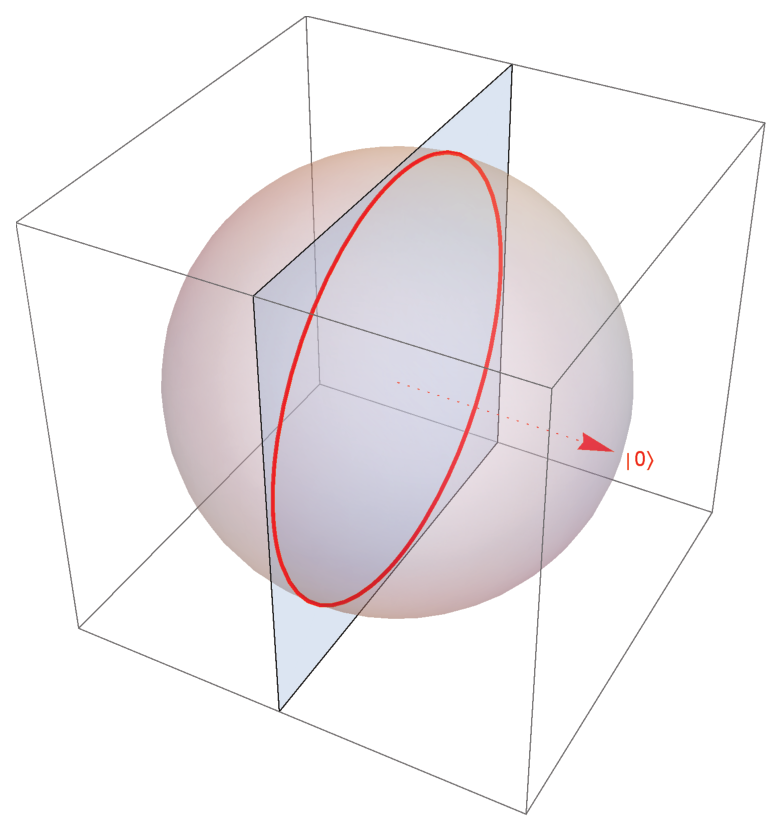
\includegraphics[scale=0.38]{figure1} 
\par\end{centering}
\caption{\label{fig:three-dimensional-3-value}This figure illustrates the
1-dimensional projectors mapped by $\bar{\mu}_{\ket{0}}^{\mathrm{B}}(P)=\iota\left(\mu_{\ket{0}}^{\mathrm{B}}(P)\right)$
plotted in $\mathbb{R}^{3}$. The red dotted vector is $\ket{0}$,
and $\bar{\mu}_{\ket{0}}^{\mathrm{B}}\left(\proj{0}\right)=\necess$. $\ket{0}$
is the normal vector of the plane so that we have $\bar{\mu}_{\ket{0}}^{\mathrm{B}}\left(\proj{\psi}\right)=\imposs$
for any vector~$\ket{\psi}$ in the plane. For any other vector~$\ket{\psi}$,
we have $\bar{\mu}_{\ket{0}}^{\mathrm{B}}\left(\proj{\psi}\right)=\unknown$.}
\end{figure}
For example, figure~\ref{fig:three-dimensional-3-value} plots the
1-dimensional projectors mapped by $\iota\left(\mu_{\ket{0}}^{\mathrm{B}}(P)\right)$.
This measure represents the beliefs of an experimenter with no prior
knowledge about the particular quantum system in question.\footnote{\yutsung{Actually, $\iota\left(\mu_{\ket{0}}^{\mathrm{B}}(P)\right)$ is quite
informative. Since $\iota\left(\mu_{\ket{0}}^{\mathrm{B}}(P)\right)=\necess$
if and only if $P=\proj{0}$, we know the core of $\iota\left(\mu_{\ket{0}}^{\mathrm{B}}(P)\right)$
is exactly $\left\{ \mu_{\ket{0}}^{\mathrm{B}}\right\} $. The quantum interval-valued
probability measure for an experimenter with no prior knowledge should
be $\bar{\mu}(P)=\unknown$ for every projection~$P$.}} 

Similarly, we can recast the result of cryptodeterminism to quantum
interval-valued probability measures as well. In another word, for
any classically event space~$\events$,there is always a classical
interval-valued probability measure~$\bar{\mu}:\events\rightarrow\left\{ \imposs,\necess\right\} $.
However, given a Hilbert space of dimension~$d\ge3$, there is no
quantum interval-valued probability measure~$\bar{\mu}:\events\rightarrow\left\{ \imposs,\necess\right\} $
by corollary~\ref{cor:Kochen-Specker-IVPM} of the Kochen-Specker
theorem. The Kochen-Specker theorem provides an example that quantum
interval-valued probability measures behave differently from the classical
one, and the convexity and core in the next section provides another
example that quantum interval-valued probability measures behave unexpectedly.

%%%%%


\subsection{Convexity and Core}

\noindent Formally, we can ask: what can we deduce about the state
of a quantum system given a quantum interval-valued probability measure,
i.e., given observations done with finite resources. In the case that
the intervals are infinitely precise, the question reduces to Gleason's
theorem which states that the state of the quantum system is uniquely
determined by the probability measure. But surely the less resources
are available, the less precise the intervals, and the less we expect
to know about the state of the system. To formally state and answer
this question we begin with defining the \emph{core} and \emph{convexity}
of a probability measure as follows.

\begin{definition} Given a quantum interval-valued probability measure~$\bar{\mu}:\events\rightarrow\mathscr{I}$: 
\begin{itemize}
\item A \emph{core} of $\bar{\mu}$ is the set $\mathrm{core}\left(\bar{\mu}\right)=\set{\pmeas:\events\rightarrow[0,1]}{\forall P\in\events.~\pmeas\left(P\right)\in\bar{\mu}\left(P\right)}$. 
\item $\bar{\mu}$ is called convex if 
\begin{equation}
\bar{\mu}\left(P_{0}\vee P_{1}\right)+\bar{\mu}\left(P_{0}P_{1}\right)\subseteq\bar{\mu}\left(P_{0}\right)+\bar{\mu}\left(P_{1}\right)\label{eq:QuantumInterval-valuedProbability-Convex}
\end{equation}
for all commuting $P_{0},P_{1}\in\events$. 
\end{itemize}
\end{definition}

\noindent The core of an interval-valued probability measure is the
set of real-valued infinitely-precise probability measures it approximates.
An interval-valued probability measure is convex if whenever certain
intervals exist then combinations of these intervals must also exist,
guaranteeing we can add and manipulate probabilities coherently. In
the classical world, every convex measure has a non-empty core, which
means that the interval-valued probability measure must approximate
at least one infinitely-precise measure.

\begin{thm}[Shapley~\cite{Shapley1971,,Grabisch2016}]\label{thm:Shapley}
Every (classical) convex interval-valued probability measure has a
non-empty core. \end{thm}

In informal terms, this result states that although measurements done
with limited resources and poor precision may not uniquely identify
the true state of the system, there is always at least one system
that is consistent with the measurements. Surprisingly, we discovered
a counterexample to this statement in the quantum case, and have:

\begin{thm}\label{def:EmptyCoreQuantumInterval-valuedProbability}
There is a convex quantum interval-valued probability measure~$\bar{\mu}:\events\rightarrow\mathscr{I}$
such that $\mathrm{core}\left(\bar{\mu}\right)=\emptyset$.\end{thm}

This theorem could be proved by constructing the following convex
quantum interval-valued probability measure with an empty core.
\begin{figure}
\begin{centering}
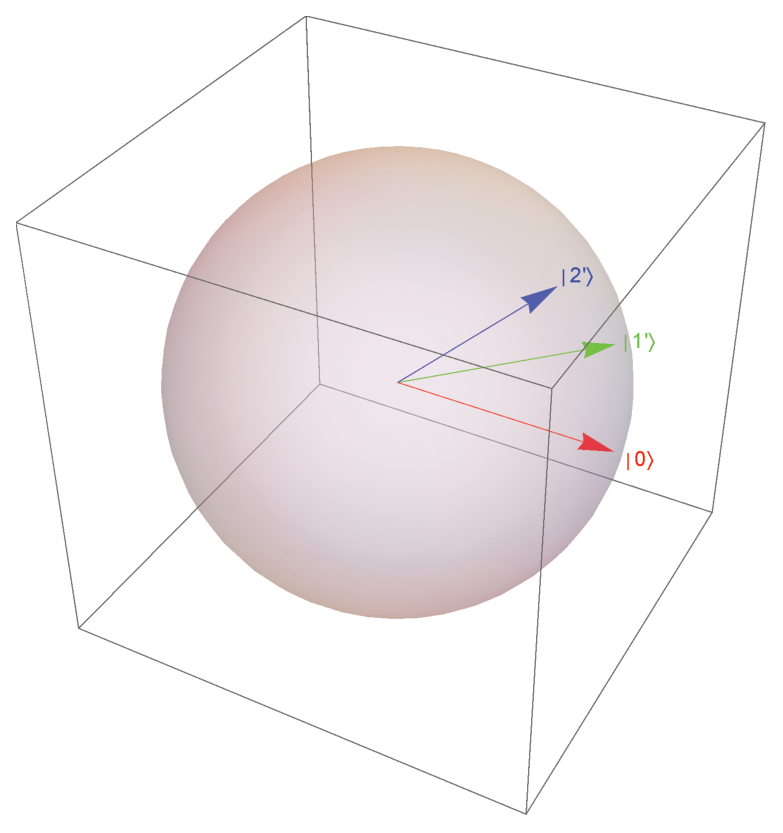
\includegraphics[scale=0.38]{figure2_1} 
\par\end{centering}
\caption{\label{fig:three-dimensional-3-value-2}This figure illustrates example~\ref{ex:three-dimensional-three-value}
plotted in $\mathbb{R}^{3}$. The red, green, and blue vectors are
$\ket{0}$, $\ket{\ps}$, and $\ket{\ps'}$ respectively. }
\end{figure}

\begin{example}[Three-dimensional quantum three-interval-valued probability
measure]\label{ex:three-dimensional-three-value} Given a three dimensional
Hilbert space with an orthonormal basis $\left\{ \ket{0},\ket{1},\ket{2}\right\} $.
Let $\mathscr{I}=\left\{ \necess,\imposs,\unknown\right\} $, $\ket{\ps}=\left(\ket{0}+\ket{1}\right)/\sqrt{2}$,
$\ket{\ps'}=\left(\ket{0}+\ket{2}\right)/\sqrt{2}$, and 
\begin{equation}\eqalign{ 
\bar{\mu}(\mathbb{0})=\bar{\mu}(\proj{0})=\bar{\mu}(\proj{\ps})=\bar{\mu}(\proj{\ps'})=\imposs\textrm{ ,}\\ 
\bar{\mu}(\mathbb{1})=\bar{\mu}(\mathbb{1}-\proj{0})=\bar{\mu}(\mathbb{1}-\proj{\ps})=\bar{\mu}(\mathbb{1}-\proj{\ps'})=\necess\textrm{ ,}\\ 
\bar{\mu}(P) = \unknown\qquad\textrm{otherwise.} 
}\end{equation}
It is straightforward to verify that $\bar{\mu}$ is a quantum interval-valued
probability measure by theorem~\ref{thm:interval-valued-frame-function}
and convex by theorem~\ref{thm:convex-3}. Now assume there exists
a real-valued quantum probability measure $\mu$ such that $\mu(P)\in\bar{\mu}(P)$
for every event (projection)~$P$. We derive a contradiction as follows.
Suppose $\mu(P)\in\bar{\mu}(P)$ then we must have $\mu(\proj{0})=\mu(\proj{\ps})=\mu(\proj{\ps'})=0$.
By Gleason's theorem, there is a mixed state~$\rho=\sum_{j=1}^{N}q_{j}\proj{\phi_{j}}$
such that $\mu\left(P\right)=\sum_{j=1}^{N}q_{j}\ip{\phi_{j}}{P\phi_{j}}$,
where $\sum_{j=1}^{N}q_{j}=1$ and $q_{j}>0$. However, no pure state~$\ket{\phi}$
can satisfy $\ip{\phi}{0}=\ip{\phi}{\ps}=\ip{\phi}{\ps'}=0$; a contradiction.
\end{example}

%%%%%%%%%%%%%%%%%%%%%%%%%%%%%%%%%%%%%%%%%%%%%%%%%%%%%%%%%%%%%%%%%%%%%%%%%%%%%%
\section{Why Empty Core?}

The possibility that a convex quantum interval-valued probability
measure has an empty core departs from the classical case. To understand
the meaning of it, we will first study how to recover the non-empty
core with extra conditions. We will then consider having an empty
core as an legitimate result, and understand its consequence.

\subsection{Convexity}

One possibility for having an empty core is that the definition of
quantum convexity is too weak. On one hand, strengthening equation~(\ref{eq:QuantumInterval-valuedProbability-Convex})
to non-commuting projectors~$P_{0}$ and $P_{1}$ is unlikely to
succeed because the product of non-commuting projectors is not a projector.
On the other hand, strengthening equation~(\ref{eq:QuantumInterval-valuedProbability-Convex})
among commuting projectors cannot guarantee a non-empty core as well
if we follow what people strengthen convexity classically. Equation~(\ref{eq:QuantumInterval-valuedProbability-Convex})
classically is a special case of 
\begin{equation}
\bar{\mu}'\left(\bigcup_{i=1}^{N}E_{i}\right)+\sum_{{{\scriptstyle I\subseteq\left\{ 1,\ldots,N\right\} }\atop {\scriptstyle \left|I\right|\textrm{ is odd}}}}\bar{\mu}'\left(\bigcap_{i\in I}E_{i}\right)\subseteq\sum_{{{\scriptstyle I\subseteq\left\{ 1,\ldots,N\right\} }\atop {\scriptstyle \left|I\right|\textrm{ is even}}}}\bar{\mu}'\left(\bigcap_{i\in I}E_{i}\right)\label{eq:Dempster-Shafer-game}
\end{equation}
when $N=2$, where $\bar{\mu}'$ is a classical interval-valued probability
measure. If $\bar{\mu}'$ satisfies equation~(\ref{eq:Dempster-Shafer-game})
for all set of event~$\left\{ E_{i}\right\} _{i=1}^{N}\subseteq2^{\Omega}$,
then the left-end point of $\bar{\mu}'$ is called a Dempster-Shafer
belief function. It is reasonable to call a quantum interval-valued
probability~$\bar{\mu}$ Dempster-Shafer if $\bar{\mu}$ satisfies
\begin{equation}
\bar{\mu}\left(\bigvee_{i=1}^{N}P_{i}\right)+\sum_{{{\scriptstyle I\subseteq\left\{ 1,\ldots,N\right\} }\atop {\scriptstyle \left|I\right|\textrm{ is odd}}}}\bar{\mu}\left(\prod_{i\in I}P_{i}\right)\subseteq\sum_{{{\scriptstyle I\subseteq\left\{ 1,\ldots,N\right\} }\atop {\scriptstyle \left|I\right|\textrm{ is even}}}}\bar{\mu}\left(\prod_{i\in I}P_{i}\right)\textrm{ .}\label{eq:Dempster-Shafer-game-quantum}
\end{equation}
for all set of mutually orthogonal projections~$\left\{ P_{i}\right\} _{i=1}^{N}\subseteq\events$.
However, the quantum interval-valued probability measure in example~\ref{ex:three-dimensional-three-value}
is Dempster-Shafer and has an empty core. In summary, it is unlikely
to guarantee a non-empty core by strengthening convexity.

\subsection{Commuting Sub-Event Space}

Another reason for having an empty core is the existence of non-commuting
observables. Non-commutativity is one of the difference between quantum
and classical since Heisenberg's uncertainty principle states there
is an intrinsic uncertainty measuring non-commuting observables in
quantum mechanics~\cite{Heisenberg1983,peres1995quantum,544199,Griffiths2003,Jaeger2007}.
Similarly, we argue that the quantum phenomenon disappears when we
restrict the domain of a quantum interval-valued probability measure~$\bar{\mu}:\events\rightarrow\mathscr{I}$
on a mutually commuting subspace~$\events'$. As proved in theorem~\ref{thm:sub-event-space},
the restricted $\bar{\mu}|_{\events'}$ is essentially a classical
interval-valued probability measure. Furthermore, if $\bar{\mu}$
is convex, then $\bar{\mu}|_{\events'}$ will be convex, and have
a non-empty core classically. 

When $\bar{\mu}$ is restricted to different commuting $\events'$,
the core elements of each $\bar{\mu}|_{\events'}$ may not be glued
together, and gives a core element of $\bar{\mu}$. The inability
of gluing core elements among commuting $\events'$ to non-commuting
$\events$ is consistent with the proof of the Kochen-Specker theorem,
where each triple of commuting observables could be colored well,
but we cannot color all observables which are not all commuting. This
is also consistent with the assertion that mutually commuting observables
could be measured simultaneously~\cite{Mermin_1993}. In another
word, if Alice and Bob in Bell's theorem can only pick from a set
of mutually commuting observables, they could never observe any ``quantum,``
and prove the quantum theory cannot be simulated by a local hidden
variable theory.

\subsection{Increase the Measurement Resource}

This section extend the idea of restricting the event space, but instead
of commuting sub-event space, we will try to find some subset~$\events'\subseteq\events$
such that $\bar{\mu}|_{\events'}$ has an non-empty core. This could
help us understand the core because of the following identity
\begin{equation}
\mathrm{core}\left(\bar{\mu}\right)=\bigcap_{\events'\subseteq\events}\mathrm{core}\left(\bar{\mu}|_{\events'}\right)\label{eq:core-intersection}
\end{equation}
if we know more about the right-hand side of the equation, we can
have more idea about the left-hand side. This idea can be applied
to example~\ref{ex:three-dimensional-three-value}, and the following
are three of all possibilities:
\begin{itemize}
\item When $\events_{1}=\events\backslash\left\{ \proj{\ps'}\right\} $,
because $\bar{\mu}(\proj{0})=\bar{\mu}(\proj{\ps})=\imposs$, we have
$\mathrm{core}\left(\bar{\mu}|_{\events_{1}}\right)=\left\{ \mu_{\ket{2}}^{\mathrm{B}}\right\} $.
\item When $\events_{2}=\events\backslash\left\{ \proj{\ps}\right\} $,
because $\bar{\mu}(\proj{0})=\bar{\mu}(\proj{\ps'})=\imposs$, we
have $\mathrm{core}\left(\bar{\mu}|_{\events_{2}}\right)=\left\{ \mu_{\ket{1}}^{\mathrm{B}}\right\} $.
\item When $\events_{3}=\events\backslash\left\{ \proj{0},\proj{\ps},\proj{\ps'}\right\} $,
because $\bar{\mu}(\proj{\phi})\ne\necess$ for all $\ket{\phi}$,
we have $\mu_{\frac{\mathbb{1}}{3}}^{\mathrm{B}}\in\mathrm{core}\left(\bar{\mu}|_{\events_{3}}\right)$
as well as $\mu_{\ket{2}}^{\mathrm{B}}$ and $\mu_{\ket{1}}^{\mathrm{B}}\in\mathrm{core}\left(\bar{\mu}|_{\events_{3}}\right)$.
\end{itemize}
Each of these possibilities is compatible with some but not all of
the observations. In another word, 
\begin{equation}
\mathrm{core}\left(\bar{\mu}\right)=\bigcap_{\events'\subseteq\events}\mathrm{core}\left(\bar{\mu}|_{\events'}\right)\subseteq\mathrm{core}\left(\bar{\mu}|_{\events_{1}}\right)\cap\mathrm{core}\left(\bar{\mu}|_{\events_{2}}\right)=\left\{ \mu_{\ket{2}}^{\mathrm{B}}\right\} \cap\left\{ \mu_{\ket{1}}^{\mathrm{B}}\right\} =\emptyset\textrm{ .}
\end{equation}
The first two possibilities are particular interesting since each
two 1-dimensional projectors~$\proj{\psi_{0}}$ and $\proj{\psi_{1}}$
mapped to $\imposs$ suggests there is a subset~$\events'\subseteq\events$
such that $\mathrm{core}\left(\bar{\mu}|_{\events'}\right)=\left\{ \mu_{\ket{\psi_{0}}\times\ket{\psi_{1}}}^{\mathrm{B}}\right\} $
in the Hilbert space of dimension 3, where the cross product of complex
vectors is defined in definition~\ref{def:cross-product}. 

As we illustrated in figure~\ref{fig:three-dimensional-3-value},
if $\bar{\mu}$ has a non-empty core, the states mapping to $\imposs$
is contained in a plane, which contains no area in the sphere. On
the other hand, if the states mapping to $\imposs$ contain some area
in the sphere as in figure~\ref{fig:three-dimensional-real-frame-1},
and this area intersects a plane~$\events'$, then $\mathrm{core}\left(\bar{\mu}|_{\events'}\right)=\left\{ \mu_{\ket{\psi}}^{\mathrm{B}}\right\} $,
where $\ket{\psi}$ is the normal vector of $\events'$. Since different
planes have different normal vectors, $\bar{\mu}$ has an empty core.
Furthermore, the larger the area, the more state vectors which are
inconsistent with any particular Born rule probability measure. In
another word, there are more different singleton sets in the right-hand
side of equation~(\ref{eq:core-intersection}). Therefore, the area
of the 1-dimensional projectors mapping to $\imposs$ could indicate
how much $\bar{\mu}$ deviate from the Born rule probability measures.

In this sense, we found that the area of the 1-dimensional projectors
mapping to $\imposs$ depends on the maximal length of the intervals,
which represents the ability of measurement equipment. In particular,
we have the following results whose details are described in \ref{sec:Real-Interval-valued-Frame}. 
\begin{itemize}
\item The radius of any disk inside the area of the 1-dimensional projectors
mapping to $\imposs$ must smaller than $\pi / 4$ (theorem~\ref{thm:pi-div-4}).
\item When the radius of any disk inside the area of the 1-dimensional projectors
mapping to $\imposs$ between $\arcsin\left(1 / \sqrt{3}\right)$
and $\pi / 4$, we have $\unknown\in\mathscr{I}$, i.e., $\underset{\left[l,r\right]\in\mathscr{I}}{\max}r-l=1$
(theorem~\ref{thm:arcsin-one-over-sqrt-three}).
\item When the radius of any disk inside the area of the 1-dimensional projectors
mapping to $\imposs$ between $\pi/6$ and $\arcsin\left(1 / \sqrt{3}\right)$,
we have $\underset{\left[l,r\right]\in\mathscr{I}}{\max}r-l=\frac{1}{3}$
(to be typed...).
\end{itemize}
In general, we conjecture that if the measurement equipment is made
more and more precise, the corresponding interval-valued probability
measure will be closer and closer to the Born rule. In the limit case,
$\mathscr{I}=\set{\left\{ a\right\} }{a\in\left[0,1\right]}$ we do
indeed recover the conventional Gleason's theorem and the Born rule.

%%%%%


\subsection{Wigner's Friends}

The situation of empty core might not be that strange if we think
in terms of Wigner's ``friends.'' In the original story of Wigner
and his friend~\cite{Wigner1961,FuchsMerminSchack2014}, the friend
makes a measurement in a closed laboratory and experiences an outcome.
Wigner, outside the laboratory, doesn't experience an outcome. If
he believes what his friend has told him about her plans in her laboratory
he will assign an entangled state to her, her apparatus, and the system
on which she is making her intervention. If Wigner goes on to ask
his friend about her experience, then the entangled state to her,
her apparatus, and the system will change into one in which they even
have separate wave functions, and Wigner and his friend will use the
same wave function to describe the system.

The question is what happens if Wigner has more than one friend in
the laboratory. Suppose Wigner has three friends: E, P, and R in the
laboratory. E, P, and R measure the spin-1 system described in example~\ref{ex:three-dimensional-three-value}.
After the experiment, E tells Wigner $\proj{0}$ never happened, P
tells Wigner $\proj{\ps}$ never happened, and R tells Wigner $\proj{\ps'}$
never happened. Wigner may then need to use the quantum Dempster-Shafer
rule(?) or other rules(?) to combine the belief told by his friends,
and the combined belief might be the quantum interval-valued probability
measure in example~\ref{ex:three-dimensional-three-value} which
has an empty core.

%%%%%%%%%%%%%%%%%%%%%%%%%%%%%%%%%%%%%%%%%%%%%%%%%%%%%%%%%%%%%%%%%%%%%%%%%%%%%%
\section{Conclusion and Discussion}

If we insist that probabilities cannot be computed to infinite precision
and are bound to be approximations represented by intervals of confidence,
then quantum states themselves can only be discussed within intervals
of confidence. Despite the fact that classically a IVPM could always
correspond to a real-valued probability measure, we found that there
may be no ``real'' infinitely-precise quantum state approximated
by a quantum IVPM as a whole. However, if a quantum IVPM is decomposed
into pieces, each piece might still be induced by a quantum state.
Moreover, our examples and Gleason's theorem summarized in table~\ref{table_long}
suggests that as the measurement resources increase, an entire quantum
IVPM could more and more likely be identified to a particular state.
\begin{table}
\caption{\label{table_long}Relation between measurement resources and
interval-valued probability measures.}
\begin{indented}
\item[]\begin{tabular}{c|cccc}
\br
Measurement resources & Lowest & \multicolumn{2}{c}{$\longleftrightarrow$} & Highest\tabularnewline
\mr
Count of $\mathscr{I}$ & $3$ & $4$ & \ldots{} & $\infty$\tabularnewline
$\sup_{\left[l,r\right]\in\mathscr{I}}\left|r-l\right|$ & $1$ & $\frac{1}{2}$ & \ldots{} & $0$\tabularnewline
Count of $\mathrm{core}\left(\bar{\mu}\right)$ & 0 & 0 &  & 1\tabularnewline
Count of states correspond to pieces of $\bar{\mu}$ & $3$ & $2$ & \ldots{} & $1$\tabularnewline
\mr
How precise we could identify a state? & Coarse & \multicolumn{2}{c}{$\longleftrightarrow$} & Precise\tabularnewline
\br
\end{tabular}
\end{indented}
\end{table}
Additional work is in progress on the following research questions:
\begin{description}
\item [{Research Question.}] Confirm that there is always a quantum IVPM
with an empty-core if the length of the intervals is bigger than zero. 
\item [{Research Question.}] Find a general method to determine how a
quantum IVPM is close to the Born rule. 
\item [{Research Question.}] Confirm that as the number and precision
of the intervals increase the quantum IVPM converges to the measure
induced by the Born rule. 
\item [{Research Question.}] Investigate the status of the theorems of
Bell and Kochen-Specker for quantum IVPM.
\end{description}
Although we discussed how a quantum IVPM could be induced from a real
quantum state, our investigation leaves an open question of whether
there exists a ``real'' entity that exists independently of measurements
and probabilities. The possibility of no ``real'' underlying state
is consistent with the elegantly recent work on Quantum Bayesianism
or QBism~\cite{FuchsSchack2013,FuchsMerminSchack2014,VonBaeyer2016},
which suggests that the quantum state is more like an interactive
system in computer science parlance. In another word, the quantum
state is subjective: each observer has a different view of the quantum
system that is consistent with their previous observations and that
allows that observer, independently of other observers, to assign
beliefs (i.e., probabilities) to possible future interactions.

%%%%%%%%%%%%%%%%%%%%%%%%%%%%%%%%%%%%%%%%%%%%%%%%%%%%%%%%%%%%%%%%%%%%%%%%%%%%%%
\ack

Anyone who has discussed this with us?

%%%%%%%%%%%%%%%%%%%%%%%%%%%%%%%%%%%%%%%%%%%%%%%%%%%%%%%%%%%%%%%%%%%%%%%%%%%%%%
\appendix

%%%%%%%%%%%%%%%%%%%%%%%%%%%%%%%%%%%%%%%%%%%%%%%%%%%%%%%%%%%%%%%%%%%%%%%%%%%%%%
\section{Interval-valued Frame Functions\label{sec:Interval-valued-Frame-Functions}}

Although quantum IVPMs in example~\ref{ex:three-dimensional-three-value}
and \ref{ex:three-dimensional-5-value} have empty cores, we might
still think that the probability measure~$\bar{\mu}$ is induced
by some states. In example~\ref{ex:three-dimensional-three-value},
the probability measure~$\bar{\mu}$ might be induced by the state
$\ket{2}$ because $\bar{\mu}(\proj{0})=\bar{\mu}(\proj{\ps})=\imposs$,
or induced by the state $\ket{1}$ because $\bar{\mu}(\proj{0})=\bar{\mu}(\proj{\ps'})=\imposs$.
In example~\ref{ex:three-dimensional-5-value}, the probability measure~$\bar{\mu}$
might be induced by the state $\ket{2}$ because $\bar{\mu}(\proj{0})=\bar{\mu}(\proj{\ps})=\imposs$.
In general, each two real 1-dimensional projectors~$\proj{\psi_{0}}$
and $\proj{\psi_{1}}$ mapping to impossible suggests $\bar{\mu}$
might be induced by the pure state~$\ket{\psi_{0}}\times\ket{\psi_{1}}$
in the Hilbert space of dimension 3.

Since a quantum IVPM is completely determined by its value on 1-dimensional
projectors in the Hilbert space of dimension 3, we could define the
interval-valued frame function to simplify the later discussion.

\begin{definition}\cite{Hatcher2001,dryden2005}~The unit sphere
in $\mathbb{R}^{d}$ is denoted by $S^{d-1}=\set{\ket{\psi}\in\mathbb{R}^{d}}{\ip{\psi}{\psi}=1}$,
while the unit sphere in $\mathbb{C}^{d}$ is denoted by $\mathbb{C}S^{d-1}=\set{\ket{\psi}\in\mathbb{C}^{d}}{\ip{\psi}{\psi}=1}$.
Since $\mathbb{C}$ is one-to-one correspondence to $\mathbb{R}^{2}$~\cite{GAMELIN2003},
$\mathbb{C}S^{d-1}$ has the same structure as $S^{2d-1}$. However,
different symbols emphasis that they are embedded in different spaces.\end{definition}

\begin{definition}\cite{gleason1957,peres1995quantum,RichmanBridges1999}~For
any quantum probability measure~$\mu$ on the Hilbert space of dimension~$d$,
we can define its \emph{frame function}~$f:\mathbb{C}S^{d-1}\rightarrow\left[0,1\right]$
by $f\left(\ket{\psi}\right)=\mu\left(\proj{\psi}\right)$. For a
quantum probability measure~$\mu_{\phi}^{\mathrm{B}}$ induced by the Born
rule, its frame function is denoted by $f_{\phi}^{\mathrm{B}}$.\end{definition}

\begin{thm}\label{thm:frame-function}\cite{gleason1957,peres1995quantum,RichmanBridges1999}~A
frame function~$f:\mathbb{C}S^{d-1}\rightarrow\left[0,1\right]$
satisfies the following properties: 
\begin{itemize}
\item $f\left(\lambda\ket{\psi}\right)=f\left(\ket{\psi}\right)$ for any
$\ket{\psi}\in\mathbb{C}S^{d-1}$ and $\lambda\in\mathbb{C}S^{0}$. 
\item For any orthonormal basis~$\left\{ \ket{\psi_{i}}\right\} _{i=0}^{2}$,
we have $1=\sum_{i=0}^{2}f\left(\ket{\psi_{i}}\right)$. 
\end{itemize}
Conversely, if a function~$f:\mathbb{C}S^{d-1}\rightarrow\left[0,1\right]$
satisfies the above properties, $f$ must be a frame function.\end{thm}

\begin{definition}For any quantum IVPM~$\bar{\mu}$ on the Hilbert
space of dimension 3, we can define an \emph{interval-valued frame
function}~$\bar{f}:\mathbb{C}S^{2}\rightarrow\mathscr{I}$ by $\bar{f}\left(\ket{\psi}\right)=\bar{\mu}\left(\proj{\psi}\right)=\left[f^{l}\left(\ket{\psi}\right),f^{r}\left(\ket{\psi}\right)\right]$,
where $f^{l}:\mathbb{C}S^{2}\rightarrow\left[0,1\right]$ and $f^{r}:\mathbb{C}S^{2}\rightarrow\left[0,1\right]$
are the left-end and the right-end of $\bar{f}$, respectively. Also,
if $f$ is the frame function of $\mu$, $\bar{f}$ is the interval-valued
frame function of $\bar{\mu}$, and $\mu$ is in the core of $\bar{\mu}$,
then we say $f$ is in the core of $\bar{f}$, and denoted by $f\in\mathrm{core}\left(\bar{f}\right)$.\end{definition}

\begin{thm}\label{thm:interval-valued-frame-function}An interval-valued
frame function~$\bar{f}:\mathbb{C}S^{2}\rightarrow\mathscr{I}$ satisfies
the following properties:
\begin{itemize}
\item $\bar{f}\left(\lambda\ket{\psi}\right)=\bar{f}\left(\ket{\psi}\right)$
for any $\ket{\psi}\in\mathbb{C}S^{2}$ and $\lambda\in\mathbb{C}S^{0}$. 
\item For any orthonormal basis~$\left\{ \ket{\psi_{i}}\right\} _{i=0}^{2}$,
we have $\left[1,1\right]-\bar{f}\left(\ket{\psi_{i}}\right)\subseteq\bar{f}\left(\ket{\psi_{j}}\right)+\bar{f}\left(\ket{\psi_{k}}\right)$,
where $i$, $j$, and $k$ are any permutations among $0$, $1$,
and $2$. 
\end{itemize}
Conversely, if a function~$\bar{f}:\mathbb{C}S^{2}\rightarrow\mathscr{I}$
satisfies the above properties, $\bar{f}$ must be an interval-valued
frame function.\end{thm}

\begin{proof} Given a quantum IVPM~$\bar{\mu}$, it is straightforward
to verify that its interval-valued frame function~$\bar{f}:\mathbb{C}S^{2}\rightarrow\mathscr{I}$
satisfies the above properties.

Conversely, given a function~$\bar{f}:\mathbb{C}S^{2}\rightarrow\mathscr{I}$
satisfying the above properties, consider $\bar{\mu}:\events\rightarrow\mathscr{I}$
defined by 
\begin{itemize}
\item $\bar{\mu}(\mathbb{0})=\left[0,0\right]$ and $\bar{\mu}(\mathbb{1})=\left[1,1\right]$. 
\item For any $\ket{\psi}\in\mathbb{C}S^{2}$, we have $\bar{\mu}\left(\proj{\psi}\right)=\bar{f}\left(\ket{\psi}\right)$
and $\bar{\mu}\left(\mathbb{1}-\proj{\psi}\right)=\left[1,1\right]-\bar{f}\left(\ket{\psi}\right)$. 
\end{itemize}
Since other conditions are trivial, we only need to verify equation~(\ref{eq:QuantumInterval-valuedProbability-Inclusion}).
First notice that $\bar{\mu}\left(P_{0}+P_{1}\right)\subseteq\bar{\mu}\left(P_{0}\right)+\bar{\mu}\left(P_{1}\right)$
implies equation~(\ref{eq:QuantumInterval-valuedProbability-Inclusion})
by induction. Second, equation~(\ref{eq:QuantumInterval-valuedProbability-Complement})
implies $\bar{\mu}\left(\mathbb{1}\right)\subseteq\bar{\mu}\left(P\right)+\bar{\mu}\left(\mathbb{1}-P\right)$.
Therefore, to prove equation~(\ref{eq:QuantumInterval-valuedProbability-Inclusion}),
it is sufficient to check 
\begin{equation}
\bar{\mu}\left(\proj{\psi_{0}}+\proj{\psi_{1}}\right)\subseteq\bar{\mu}\left(\proj{\psi_{0}}\right)+\bar{\mu}\left(\proj{\psi_{1}}\right)
\end{equation}
for orthogonal $\ket{\psi_{0}}$ and $\ket{\psi_{1}}$,which always
holds because the properties of $\bar{f}$.\end{proof}
\begin{definition}\label{def:cross-product}For $\ket{\psi}=\alpha_{0}\ket{0}+\alpha_{1}\ket{1}+\alpha_{2}\ket{2}=\left(\begin{array}{c}
\alpha_{0}\\
\alpha_{1}\\
\alpha_{2}
\end{array}\right)$ and $\ket{\phi}=\beta_{0}\ket{0}+\beta_{1}\ket{1}+\beta_{2}\ket{2}=\left(\begin{array}{c}
\beta_{0}\\
\beta_{1}\\
\beta_{2}
\end{array}\right)$, their cross product is defined as follow: 
\begin{equation}
\ket{\psi\times\phi}=\ket{\psi}\times\ket{\phi}=\left|\begin{array}{cc}
\alpha_{1}^{*} & \beta_{1}^{*}\\
\alpha_{2}^{*} & \beta_{2}^{*}
\end{array}\right|\ket{0}+\left|\begin{array}{cc}
\alpha_{2}^{*} & \beta_{2}^{*}\\
\alpha_{0}^{*} & \beta_{0}^{*}
\end{array}\right|\ket{1}+\left|\begin{array}{cc}
\alpha_{0}^{*} & \beta_{0}^{*}\\
\alpha_{1}^{*} & \beta_{1}^{*}
\end{array}\right|\ket{2}\textrm{ ,}
\end{equation}
where $\left|\begin{array}{cc}
\alpha & \beta\\
\alpha' & \beta'
\end{array}\right|=\alpha\beta'-\alpha'\beta$. Also, even if $\ket{\psi}$ and $\ket{\phi}$ are normalized, their
cross product~$\ket{\psi}\times\ket{\phi}$ need not be normalized
as usual. We will use $\ket{\psi}\times\ket{\phi}$ and $\ket{\psi}\times\ket{\phi}/\left\Vert \ket{\psi}\times\ket{\phi}\right\Vert $
interchanged when there is no confusion.\end{definition}

\begin{definition}For $\ket{\psi}$ and $\ket{\phi}\in\mathbb{C}^{3}$,
if $\ket{\psi}=\lambda\ket{\phi}$ for some~$\lambda\ne0$, we call
$\ket{\psi}$ is parallel to $\ket{\phi}$ denoted by $\ket{\psi}\parallel\ket{\phi}$.
In this case, $\ket{\psi}$ and $\ket{\phi}$ represent the same physical
state. ``$\ket{\psi}$ is not parallel to $\ket{\phi}$'' is denoted
by $\ket{\psi}\nparallel\ket{\phi}$.\end{definition}

\begin{lemma}Given $\ket{\psi}$, $\ket{\phi}$ and $\ket{\varphi}\in\mathbb{C}^{3}$
such that $\ket{\psi}\nparallel\ket{\phi}$. Then, $\ket{\varphi}\parallel\left(\ket{\psi}\times\ket{\phi}\right)$
if and only if $\ip{\psi}{\varphi}=\ip{\phi}{\varphi}=0$.\end{lemma}
\begin{proof}
To prove that $\ket{\varphi}\parallel\left(\ket{\psi}\times\ket{\phi}\right)\Rightarrow\ip{\psi}{\varphi}=\ip{\phi}{\varphi}=0$,
we can just verify 
\begin{equation}\eqalign{
&\ip{\psi}{\psi\times\phi}=\ip{\psi\times\phi}{\psi}^{*}\\
=&\left[\left(\alpha_{1}\beta_{2}-\alpha_{2}\beta_{1}\right)\alpha_{0}+\left(\alpha_{2}\beta_{0}-\alpha_{0}\beta_{2}\right)\alpha_{1}+\left(\alpha_{0}\beta_{1}-\alpha_{1}\beta_{0}\right)\alpha_{2}\right]^{*}=0\textrm{ ,}\\
&\ip{\phi}{\psi\times\phi}=\ip{\psi\times\phi}{\phi}^{*}\\
=&\left[\left(\alpha_{1}\beta_{2}-\alpha_{2}\beta_{1}\right)\beta_{0}+\left(\alpha_{2}\beta_{0}-\alpha_{0}\beta_{2}\right)\beta_{1}+\left(\alpha_{0}\beta_{1}-\alpha_{1}\beta_{0}\right)\beta_{2}\right]^{*}=0\textrm{ .}
}\end{equation}

To prove the other direction, consider the linear transformation~$T:\mathbb{C}^{3}\rightarrow\mathbb{C}^{2}$
defined by $T\left(\ket{\varphi}\right)=\left(\begin{array}{c}\ip{\psi}{\varphi}\\
\ip{\phi}{\varphi}
\end{array}\right)$. Since $\ket{\psi}\nparallel\ket{\phi}$, we have $\mathrm{rank}\left(T\right)=2$.
Together with the rank equation~\cite{FraleighBeauregard1995}, we
have
\begin{equation}
\dim\left(\ker T\right)=\mathrm{nullity}\left(T\right)=3-\mathrm{rank}\left(T\right)=3-2=1\textrm{ .}
\end{equation}
By the other direction of the proof, we have already known $\ket{\psi}\times\ket{\phi}\in\ker T$.
Therefore, $\ket{\varphi}\parallel\left(\ket{\psi}\times\ket{\phi}\right)$.
\end{proof}
Since interval-valued probability measures~$\bar{\mu}$ and interval-valued
frame functions~$\bar{f}$ are one-to-one correspondence, studying
1-dimensional projectors mapping to impossible by $\bar{\mu}$ is
the same as studying the points on $\mathbb{C}S^{2}$ mapping to impossible
by $\bar{f}$. These points, denoted by $\bar{f}^{-1}\left(\imposs\right)=\set{\ket{\psi}\in\mathbb{C}S^{2}}{\bar{f}(\ket{\psi})=\imposs}$,
play an important role to understand $\bar{f}$. There are 4 different
cases when analyzing $\bar{f}^{-1}\left(\imposs\right)$:
\begin{enumerate}
\item $\bar{f}^{-1}\left(\imposs\right)=\emptyset$. If $f_{\phi}^{\mathrm{B}}\in\mathrm{core}\left(\bar{f}\right)$
for some pure state~$\ket{\phi}$, we could say nothing about $\ket{\phi}$.
\item $\bar{f}^{-1}\left(\imposs\right)=\left\{ \ket{\psi_{0}}\right\} $.
If $f_{\phi}^{\mathrm{B}}\in\mathrm{core}\left(\bar{f}\right)$ for some pure
state~$\ket{\phi}$, $\ket{\phi}$ could be any state orthogonal
to $\ket{\psi_{0}}$.
\item Consider $\left\{ \ket{\psi_{0}},\ket{\psi_{1}}\right\} \subseteq\bar{f}^{-1}\left(\imposs\right)$.
If $\left(\ket{\psi_{0}}\times\ket{\psi_{1}}\right)\parallel\left(\ket{\psi_{0}'}\times\ket{\psi_{1}'}\right)$
for any $\left\{ \ket{\psi_{0}'},\ket{\psi_{1}'}\right\} \subseteq\bar{f}^{-1}\left(\imposs\right)$,
then $\ket{\psi_{0}}\times\ket{\psi_{1}}$ is the only pure state
which might induce $\bar{f}$. In another word, if $f_{\phi}^{\mathrm{B}}\in\mathrm{core}\left(\bar{f}\right)$
for some pure state~$\ket{\phi}$, then $\ket{\phi}\parallel\left(\ket{\psi_{0}}\times\ket{\psi_{1}}\right)$.
For example, example~\ref{ex:three-dimensional-5-value} is in this
case when the core is empty; an interval-valued frame function defined
by $\bar{f}\left(\ket{\psi}\right)=\iota\left(f_{\phi}^{\mathrm{B}}\left(\ket{\psi}\right)\right)$
is also in this case when the core is the singleton set~$\left\{ f_{\phi}^{\mathrm{B}}\right\} $,
where $\iota$ is defined in equation~(\ref{eq:homomorphism}). 
\item If there exist two pair of states and $\left\{ \ket{\psi_{0}},\ket{\psi_{1}}\right\} $
and $\left\{ \ket{\psi_{0}'},\ket{\psi_{1}'}\right\} \subseteq\bar{f}^{-1}\left(\imposs\right)$
such that $\left(\ket{\psi_{0}}\times\ket{\psi_{1}}\right)\nparallel\left(\ket{\psi_{0}'}\times\ket{\psi_{1}'}\right)$,
then both $\ket{\psi_{0}}\times\ket{\psi_{1}}$ and $\ket{\psi_{0}'}\times\ket{\psi_{1}'}$
might induce $\bar{f}$. However, neither $f_{\psi_{0}\times\psi_{1}}^{\mathrm{B}}$
nor $f_{\psi_{0}'\times\psi_{1}'}^{\mathrm{B}}$ is in the core of $\bar{f}$
because $f_{\psi_{0}\times\psi_{1}}^{\mathrm{B}}$ is inconsistent with $\bar{f}\left(\ket{\psi_{0}'}\right)=\bar{f}\left(\ket{\psi_{1}'}\right)=\imposs$
and $f_{\psi_{0}'\times\psi_{1}'}^{\mathrm{B}}$ is inconsistent with $\bar{f}\left(\ket{\psi_{0}}\right)=\bar{f}\left(\ket{\psi_{1}}\right)=\imposs$.
Actually, $\bar{f}$ has an empty core, and this is the case for example~\ref{ex:three-dimensional-three-value}.
\end{enumerate}
In summary, if we have an idea of $\bar{f}^{-1}\left(\imposs\right)$,
we could have some idea of the pure states in core.

%%%%%%%%%%%%%%%%%%%%%%%%%%%%%%%%%%%%%%%%%%%%%%%%%%%%%%%%%%%%%%%%%%%%%%%%%%%%%%
\section{Real Interval-valued Frame Functions\label{sec:Real-Interval-valued-Frame}}

In order to simplify the discussion, we call a function~$\bar{f}:S^{2}\rightarrow\mathscr{I}$
satisfying conditions in theorem~\ref{thm:interval-valued-frame-function}
a real interval-valued frame function. Obviously, any results in appendix~\ref{sec:Interval-valued-Frame-Functions}
still hold if we replace every ``complex'' by ``real,'' in particular,
replace every $\mathbb{C}S^{2}$ by $S^{2}$. Furthermore, since restricting
the domain of a complex interval-valued frame function to $S^{2}$
gives a real interval-valued frame function, if we prove there is
no real interval-valued frame function satisfying a condition, then
there must be no complex interval-valued frame function satisfying
the corresponding condition. From now on, when we write an interval-valued
frame function~$\bar{f}$ without other specification, we would always
means a real interval-valued frame function~$\bar{f}:S^{2}\rightarrow\mathscr{I}$.

If $\bar{f}$ has a non-empty core, $\bar{f}$ must be in the case
1 - 3 in the end of appendix~\ref{sec:Interval-valued-Frame-Functions}
so that $\bar{f}^{-1}\left(\imposs\right)$ contains no area in $S^{2}$.
In contrast, if $\bar{f}^{-1}\left(\imposs\right)$ contains some
area in $S^{2}$, it must be the situation of case 4, and $\bar{f}$
has an empty core. Furthermore, the larger the area, the more state
vectors which are inconsistent with any particular Born rule frame
function. Therefore, the area of $\bar{f}^{-1}\left(\imposs\right)$
could indicate how much $\bar{f}$ deviate from the Born rule frame
functions. In the following paragraphs, we will establish that if
the area of $\bar{f}^{-1}\left(\imposs\right)$ is big, then the interval~$\mathscr{I}$
must be coarse. In another word, if the interval~$\mathscr{I}$ is
finer, then the area of $\bar{f}^{-1}\left(\imposs\right)$ would
be smaller so that $\bar{f}$ is closer to a Born rule frame function.

In order to simplify the discussion, consider the center of $\bar{f}^{-1}\left(\imposs\right)$
as the north pole, and assume $\bar{f}$ maps every state whose latitude
is larger than $\theta_{0}$ to impossible.

\begin{definition}Given a vector~$\ket{\psi}\in S^{2}$ with a specified
north pole~$\ket{0}\in S^{2}$, then $\angle\left(\ket{\psi}\right)=\arccos\ip{0}{\psi}$
denotes the latitude of $\ket{\psi}$. Conversely, $\angle^{-1}\left(I\right)=\set{\ket{\psi}\in S^{2}}{\angle\left(\ket{\psi}\right)\in I}$.
For example, the north pole has the latitude $0$, the equator has
the the latitude $\pi / 2$, and $\angle^{-1}\left(\left[0,\theta_{0}\right]\right)=\set{\ket{\psi}\in S^{2}}{\theta_{0}\le\angle\left(\ket{\psi}\right)\le\pi / 2}$
contains all states whose latitude is larger than $\theta_{0}$.\end{definition}

\begin{lemma}\label{lemma:imposs-imply-same-value}Given
$\theta_{0}\in\left[0,\pi/2\right]$ and an interval-valued frame function~$\bar{f}:S^{2}\rightarrow\mathscr{I}$,
if $\bar{f}\left(\ket{\psi}\right)=\imposs$ for every $\ket{\psi}\in\angle^{-1}\left(\left[0,\theta_{0}\right]\right)$,
then there is $l_{0}\in\left[0,\frac{1}{2}\right]$ such that $\bar{f}\left(\ket{\psi_{0}}\right)=\left[l_{0},1-l_{0}\right]\in\mathscr{I}$
for any $\ket{\psi_{0}}\in\angle^{-1}\left(\left[\pi/2-\theta_{0},\pi/2\right]\right)$.\end{lemma}
\begin{figure}
\begin{centering}
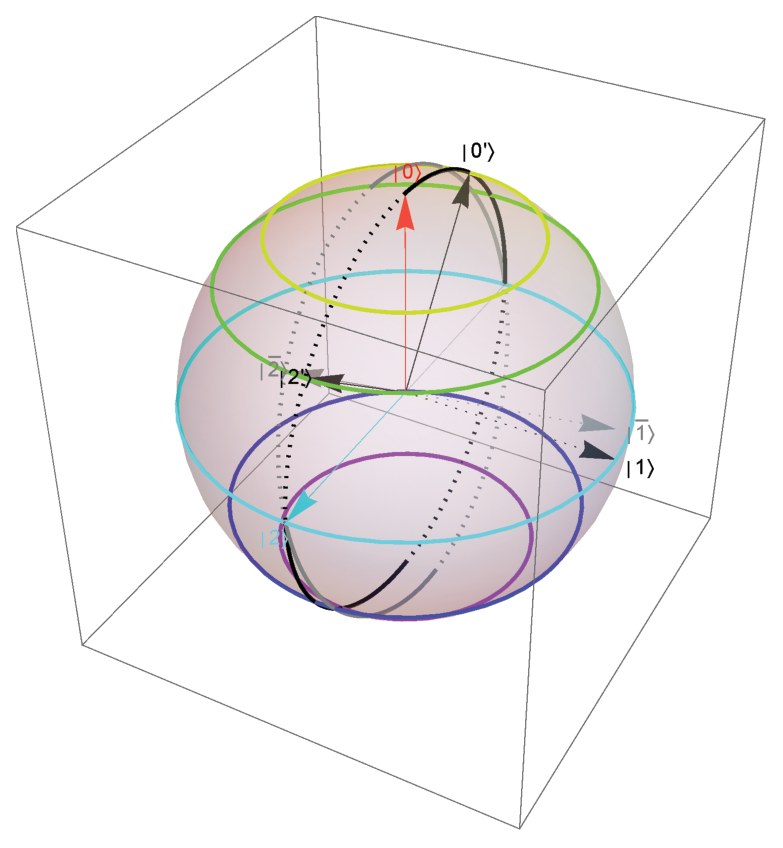
\includegraphics[scale=0.38]{figureb1} 
\par\end{centering}
\caption{\label{fig:three-dimensional-real-frame-1}This figure is used in
the proof of lemma~\ref{lemma:imposs-imply-same-value}, where every
vector above the light green circle maps to $\imposs$, and we want
to prove that every vector between dark green and light blue maps
to the same interval.}
\end{figure}
\begin{proof} We could illustrate the situation in figure~\ref{fig:three-dimensional-real-frame-1}.
Let the yellow circle is the states whose latitude is $\theta_{0}$.
Then, every states above the yellow circle maps to $\imposs$ by $\bar{f}$.
In particular, $\bar{f}\left(\ket{0}\right)=\bar{f}\left(\ket{0'}\right)=\imposs$.
Since $\left\{ \ket{0'},\ket{1},\ket{2'}\right\} $ is an orthonormal
basis, by theorem~\ref{thm:interval-valued-frame-function}, we have

\begin{equation} 
\eqalign{\left[1,1\right]-\bar{f}\left(\ket{1}\right)\subseteq\bar{f}\left(\ket{0'}\right)+\bar{f}\left(\ket{2}\right)=\bar{f}\left(\ket{2'}\right)\\ 
\left[1,1\right]-\bar{f}\left(\ket{2'}\right)\subseteq\bar{f}\left(\ket{0'}\right)+\bar{f}\left(\ket{1}\right)=\bar{f}\left(\ket{1}\right) 
} 
\label{eq:includes} 
\end{equation}
so that $\bar{f}\left(\ket{2'}\right)=\left[1,1\right]-\bar{f}\left(\ket{1}\right)$.
By the same reason, for any state~$\ket{\psi}$ in the dotted black
circle between $\ket{2'}$ and $\ket{2}$, we have $\bar{f}\left(\ket{\psi}\right)=\left[1,1\right]-\bar{f}\left(\ket{1}\right)=\bar{f}\left(\ket{2'}\right)$.
Since the angle between $\ket{0}$ and $\ket{0'}$ is the same as
the angle between $\ket{2}$ and $\ket{2'}$, for any $\ket{\psi_{0}}$
and $\ket{\psi_{1}}\in\angle^{-1}\left(\left[0,\theta_{0}\right]\right)$,
if $\ket{\psi_{0}}$ and $\ket{\psi_{1}}$ are in the same longitude,
then $\bar{f}\left(\ket{\psi_{0}}\right)=\bar{f}\left(\ket{\psi_{1}}\right)$.

Moreover, the same argument can apply on the great circle which is
not longitude. Since $\ket{\bar{1}}$ is the normal vector of the
gray circle which includes $\ket{2}$ and $\ket{\bar{2}}$, we have
$\bar{f}\left(\ket{2}\right)=\left[1,1\right]-\bar{f}\left(\ket{\bar{1}}\right)=\bar{f}\left(\ket{\bar{2}}\right)$.
In another words, for any $\ket{\psi_{0}}$ and $\ket{\psi_{1}}\in\angle^{-1}\left(\left[\pi / 2-\theta_{0},\pi / 2\right]\right)$,
even if $\ket{\psi_{0}}$ and $\ket{\psi_{1}}$ are not in the same
longitude, then $\bar{f}\left(\ket{\psi_{0}}\right)$ and $\bar{f}\left(\ket{\psi_{1}}\right)$
are still the same.

Thus, we could plug $\bar{f}\left(\ket{1}\right)=\bar{f}\left(\ket{2'}\right)=\left[l_{0},r_{0}\right]$
into equation~(\ref{eq:includes}), and get 
\begin{equation}
\left[1-r_{0},1-l_{0}\right]=\left[1,1\right]-\left[l_{0},r_{0}\right]=\left[l_{0},r_{0}\right]\Rightarrow
l_{0}+r_{0}=1\textrm{ .}
\end{equation}
Also, we have 
\begin{equation}
1\in\bar{f}\left(\ket{0'}\right)+\bar{f}\left(\ket{1}\right)+\bar{f}\left(\ket{2'}\right)=\left[2l_{0},2r_{0}\right]\Rightarrow
l_{0}\le\frac{1}{2}\le r_{0}\textrm{ .}
\end{equation}
Thus the lemma is proved.
\end{proof}
\begin{thm}\label{thm:pi-div-4}Given $\theta_{0}\in\left[0,\pi / 2\right]$
and an interval-valued frame function~$\bar{f}:S^{2}\rightarrow\mathscr{I}$,
if $\bar{f}\left(\ket{\psi}\right)=\imposs$ for every $\ket{\psi}\in\angle^{-1}\left(\left[0,\theta_{0}\right]\right)$,
then $\theta_{0}<\pi / 4$.\end{thm}
\begin{proof}
We are going to prove by contradiction. Suppose $\theta_{0}\ge\pi / 4$,
we have $\left[0,\theta_{0}\right]\cap\left[\pi / 2-\theta_{0},\pi / 2\right]=\left[\pi / 2-\theta_{0},\theta_{0}\right]\ne\emptyset$.
Pick any $\ket{\psi_{0}}\in\angle^{-1}\left(\left[\pi / 2-\theta_{0},\theta_{0}\right]\right)$,
by lemma~\ref{lemma:imposs-imply-same-value}, we have $\imposs=\bar{f}\left(\ket{\psi_{0}}\right)=\left[l_{0},1-l_{0}\right]$,
where $l_{0}\in\left[0,\pi / 2\right]$. A contradiction!
\end{proof}
\begin{thm}\label{thm:arcsin-one-over-sqrt-three}Given $\theta_{0}\in\left[\arcsin\left(1 / \sqrt{3}\right),\pi / 4\right)$
and an interval-valued frame function~$\bar{f}:S^{2}\rightarrow\mathscr{I}$,
if $\bar{f}\left(\ket{\psi}\right)=\imposs$ for every $\ket{\psi}\in\angle^{-1}\left(\left[0,\theta_{0}\right]\right)$,
then $\unknown\in\mathscr{I}$.\end{thm}
\begin{figure}
\begin{centering}
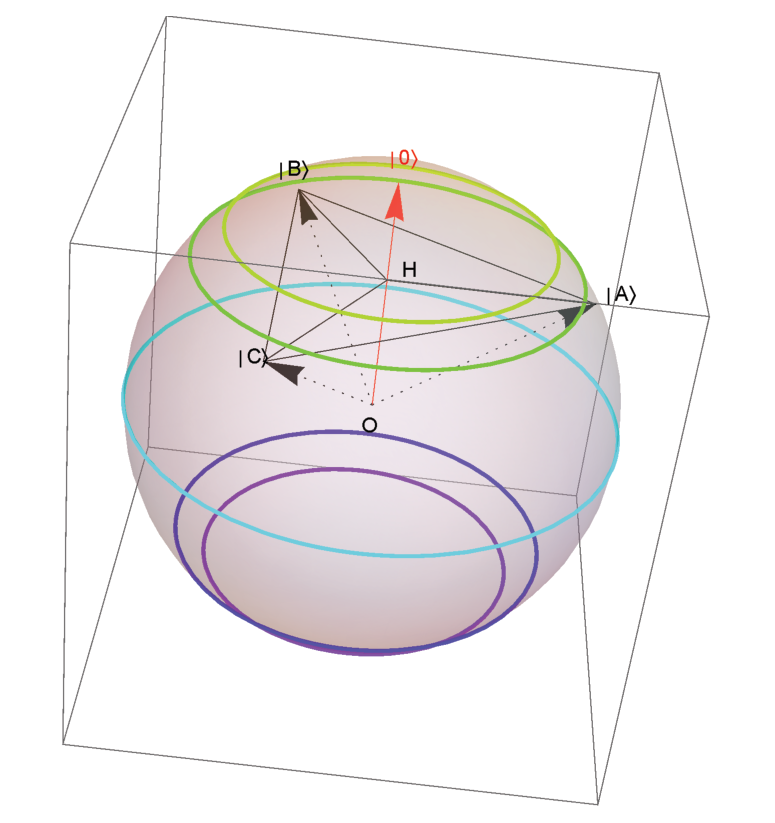
\includegraphics[scale=0.38]{figureb2.eps} 
\par\end{centering}
\caption{\label{fig:three-dimensional-real-frame-2}This figure is used in
the proof of theorem~\ref{thm:arcsin-one-over-sqrt-three}. The latitude
of the yellow circle is $\theta_{0}\in\left[\arcsin\left(1 / \sqrt{3}\right),\pi / 4\right)$,
and the latitude of the green circle is $\pi / 2-\theta_{0}$.}
\end{figure}
\begin{proof}
We could illustrate the situation in figure~\ref{fig:three-dimensional-real-frame-2},
where the latitude of of the yellow circle is $\theta_{0}$ and the
latitude of of the green circle is $\pi / 2-\theta_{0}$. Therefore,
$\bar{f}$ should map any state above the yellow circle to $\imposs$
and any states between the green circle and the equator to the same
interval, say, $\left[l_{0},1-l_{0}\right]$, where $0\le l_{0}\le\frac{1}{2}$
by lemma~\ref{lemma:imposs-imply-same-value}.

When $\theta_{0}\ge\arcsin\left(1 / \sqrt{3}\right)$, the latitude
of the green circle is $\theta_{0}\le\pi / 2-\arcsin\left(1 / \sqrt{3}\right)$.
Now consider three states~$\ket{A}$, $\ket{B}$, and $\ket{C}$
whose latitude is $\pi / 2-\arcsin\left(1 / \sqrt{3}\right)$
so that they are below the green circle, and these three states form
an equilateral triangle whose center is $H$. Since the latitude of
this triangle is $\pi / 2-\arcsin\left(1 / \sqrt{3}\right)$,
we know $\overline{OH}=1 / \sqrt{3}$, where $O$ is the center
of the sphere. By the Pythagorean theorem, $\overline{HA}=\overline{HB}=\sqrt{\frac{2}{3}}$.
Notice that $\triangle HAB$ is an isosceles triangle with $\angle AHB=2\pi / 3$,
we have $\overline{AB}=\sqrt{2}$. Since $\overline{OA}=\overline{OB}=1$
and $\overline{AB}=\sqrt{2}$, $\triangle OAB$ is an isosceles right
triangle with $\angle AHB=\pi / 2$, i.e., $\ket{A}$ and $\ket{B}$
are orthogonal. Applying the same reason on all $\ket{A}$, $\ket{B}$,
and $\ket{C}$, $\left\{ \ket{A},\ket{B},\ket{C}\right\} $ is an
orthonormal basis.

Since $\left\{ \ket{A},\ket{B},\ket{C}\right\} $ is an orthonormal
basis and $\bar{f}\left(\ket{A}\right)=\bar{f}\left(\ket{B}\right)=\bar{f}\left(\ket{C}\right)=\left[l_{0},1-l_{0}\right]$,
we have the following inequalities by theorem~\ref{thm:interval-valued-frame-function},
\begin{equation}
\left[1,1\right]-\left[l_{0},1-l_{0}\right]\subseteq\left[2l_{0},2-2l_{0}\right]\Rightarrow l_{0}\le0\textrm{ .}
\end{equation}
Recall that $0\le l_{0}\le\frac{1}{2}$. Therefore, $l_{0}=0$, that
is, $\unknown=\left[l_{0},1-l_{0}\right]\in\mathscr{I}$. \end{proof}

%%%%%%%%%%%%%%%%%%%%%%%%%%%%%%%%%%%%%%%%%%%%%%%%%%%%%%%%%%%%%%%%%%%%%%%%%%%%%%
\section{Between Quantum and Classical}

This section discusses the relation between quantum and classical.
We first prove that any quantum phenomenon would not be observed if
we could only access commuting projectors since commuting projectors
could be measured simultaneously~\cite{Mermin_1993}. Based on this
fact, we show a quantum IVPM~$\bar{\mu}$ is convex if its restriction
on any orthonormal basis~$\Omega$, $\bar{\mu}^{\Omega}$, is a convex
classical IVPM. Together with the fact that every classical IVPM~$\bar{\mu}^{\Omega}$
is convex when the number of elements in $\Omega\le3$, every quantum
IVPM must be convex on a three-dimensional Hilbert space. 

Before diving into the lemmas and proofs, we start from two definitions.

\begin{definition}Given a Hilbert space $\Hilb$, and a set of projections
$\mathcal{S}\subseteq\events$, we define $\sum_{P\in\mathcal{S}}P=\mathbb{0}$
when $\mathcal{S}=\emptyset$ since $\mathbb{0}$ is the additive
identity in operators.\end{definition}

\begin{definition}\label{definition:quantum-classical}Given a Hilbert
space $\Hilb$ with an orthonormal basis~$\Omega=\left\{ \ket{j}\right\} _{j=0}^{d-1}$.
\begin{itemize}
\item For any quantum probability measure~$\mu:\events\rightarrow\left[0,1\right]$,
we define $\mu^{\Omega}:2^{\Omega}\rightarrow\left[0,1\right]$ by
$\mu^{\Omega}\left(E\right)=\mu\left(\sum_{\ket{j}\in E}\proj{j}\right)$.
\item For any quantum IVPM~$\bar{\mu}:\events\rightarrow\mathscr{I}$,
we define $\bar{\mu}^{\Omega}:2^{\Omega}\rightarrow\mathscr{I}$ by
$\bar{\mu}^{\Omega}\left(E\right)=\bar{\mu}\left(\sum_{\ket{j}\in E}\proj{j}\right)$.
\end{itemize}
\end{definition}

\begin{lemma}\label{lemma:classical-probability-measures}$\mu^{\Omega}$
and $\bar{\mu}^{\Omega}$ in the previous definition are classical
real-valued and interval-valued probability measures, respectively.\end{lemma}

\begin{proof}When $\mathscr{I}=\set{\left\{ a\right\} }{a\in\left[0,1\right]}$,
$\bar{\mu}$ and $\bar{\mu}^{\Omega}$ are essentially quantum and
classical real-valued probability measures, respectively. Hence, it
is sufficient to prove the interval-valued case.
\begin{itemize}
\item $\bar{\mu}^{\Omega}(\emptyset)=\bar{\mu}\left(\sum_{\ket{j}\in\emptyset}\proj{j}\right)=\bar{\mu}\left(\mathbb{0}\right)=[0,0]$. 
\item $\bar{\mu}^{\Omega}(\Omega)=\bar{\mu}\left(\sum_{\ket{j}\in\Omega}\proj{j}\right)=\bar{\mu}\left(\mathbb{1}\right)=[1,1]$. 
\item For any event $E\in2^{\Omega}$,
\begin{equation}
\bar{\mu}^{\Omega}\left(\Omega\backslash E\right)=\bar{\mu}\left(\mathbb{1}-\sum_{\ket{j}\in E}\proj{j}\right)=\bar{\mu}\left(\mathbb{1}\right)-\bar{\mu}\left(\sum_{\ket{j}\in E}\proj{j}\right)=\left[1,1\right]-\bar{\mu}^{\Omega}\left(E\right)\textrm{ .}
\end{equation}
\item For a collection $\left\{ E_{i}\right\} _{i=1}^{N}\subseteq2^{\Omega}$
of pairwise disjoint events, we have
\begin{equation}
\bar{\mu}^{\Omega}\left(\bigcup_{i=1}^{N}E_{i}\right)=\bar{\mu}\left(\sum_{i=1}^{N}\sum_{\ket{j}\in E_{i}}\proj{j}\right)\subseteq\sum_{i=1}^{N}\bar{\mu}\left(\sum_{\ket{j}\in E_{i}}\proj{j}\right)=\sum_{i=1}^{N}\bar{\mu}^{\Omega}\left(E_{i}\right)\textrm{ .}
\end{equation}
\end{itemize}
\end{proof}

\begin{definition}\label{def:sub-event-space}Given a Hilbert space
$\Hilb$, $\events'\subseteq\events$ is called a sub-event space
if it satisfies the follow conditions.
\begin{itemize}
\item $\mathbb{0}\in\events'$.
\item $\mathbb{1}\in\events'$.
\item For any projection $P\in\events'$, we have $\mathbb{1}-P\in\events'$.
\item For a set of mutually orthogonal projections $\left\{ P_{i}\right\} _{i=1}^{N}\subseteq\events'$,
we have $\sum_{i=1}^{N}P_{i}\in\events'$.
\end{itemize}
By replacing every occurrence of $\events$ by $\events'$ in definition~\ref{def:QuantumCryptodeterministicMeasures},
\ref{def:QuantumProbabilitySpace}, and \ref{def:QuantumInterval-valuedProbability},
it is straightforward to define a quantum cryptodeterministic, real-valued
probability, and interval-valued probability measure on $\events'$.\end{definition}

\begin{thm}\label{thm:sub-event-space}Given a Hilbert space~$\Hilb$
and a mutually commuting sub-event space~$\events'\subseteq\events$,
there is set~$\Omega$ and a function~$\tau:\events'\rightarrow2^{\Omega}$
such that:
\begin{itemize}
\item If $\mu:\events'\rightarrow\left[0,1\right]$ is a quantum real-valued
probability measure, then there is a classical real-valued probability
measure~$\mu':\Omega\rightarrow\left[0,1\right]$ such that $\mu\left(P\right)=\mu'\left(\tau\left(P\right)\right)$
for all $P\in\events'$.
\item If $\bar{\mu}:\events'\rightarrow\mathscr{I}$ is a quantum interval-valued
probability measure, then there is a classical interval-valued probability
measure~$\bar{\mu}':\Omega\rightarrow\mathscr{I}$ such that $\bar{\mu}\left(P\right)=\bar{\mu}'\left(\tau\left(P\right)\right)$
for all $P\in\events'$
\end{itemize}
\end{thm}

\begin{proof}Again, it is sufficient to prove the interval-valued
case. Since $\events'$ is a set of mutually orthogonal projections,
they can be diagonalized by a common orthonormal basis~$\Omega=\left\{ \ket{j}\right\} _{j=0}^{d-1}$.
Pick arbitrary projector~$P\in\events'$, its eigenvalues are $0$
or $1$. Let $\tau\left(P\right)\subseteq\Omega$ be the set of eigenvectors
whose eigenvalues are $1$. Then, we have $P=\sum_{\ket{j}\in\tau\left(P\right)}\proj{j}$.
By definition~\ref{definition:quantum-classical}, $\bar{\mu}\left(P\right)=\bar{\mu}^{\Omega}\left(\tau\left(P\right)\right)$,
and $\bar{\mu}^{\Omega}$ is a quantum interval-valued probability
measure by lemma~\ref{lemma:classical-probability-measures}.\end{proof}

Given an orthonormal basis~$\Omega=\left\{ \ket{j}\right\} _{j=0}^{d-1}$,
if we consider sub-event space generated by $\Omega$, $\events^{\Omega}=\set{\sum_{\ket{j}\in E}\proj{j}}{E\subseteq\Omega}$,
then any quantum IVPM~$\bar{\mu}:\events\rightarrow\mathscr{I}$
restricting on $\events^{\Omega}$, denoted by $\bar{\mu}|_{\events^{\Omega}}$,
behaves classically. In particular, if $\bar{\mu}$ is convex, each
$\bar{\mu}|_{\events^{\Omega}}$ is convex and has a non-empty core.
However, the core elements of each $\bar{\mu}|_{\events^{\Omega}}$
may not be glued together, and gives a core element of $\bar{\mu}$.
The inability of gluing core elements among commuting $\events^{\Omega}$
to non-commuting $\events$ is consistent with the idea of the Kochen-Specker
theorem, that each triple of commuting observables could be colored
well, but we cannot color all observables which are not all commuting.
This is also consistent with the assertion that mutually commuting
observables could be measured simultaneously~\cite{Mermin_1993}.
In another word, if Alice and Bob in Bell's theorem can only pick
from a set of mutually commuting observables, they could never observe
any ``quantum,`` and we cannot eliminate the local hidden variable
theory in this setting.

The rest of the section focus on convexity.

\begin{lemma}Given a quantum IVPM~$\bar{\mu}:\events\rightarrow\mathscr{I}$,
if $\bar{\mu}^{\Omega}:2^{\Omega}\rightarrow\mathscr{I}$ are all
convex for any orthonormal basis~$\Omega$, then $\bar{\mu}$ is
convex.\end{lemma}

\begin{proof} Pick two commuting events~$P_{0},P_{1}\in\events$.
Since they are commuting, they can be diagonalized by a common orthonormal
basis~$\Omega=\left\{ \ket{j}\right\} _{j=0}^{d-1}$. Since they
are projectors, the eigenvalues of them are $0$ or $1$ so that we
can express them as $P_{0}=\sum_{\ket{j}\in E_{0}}\proj{j}$ and $P_{1}=\sum_{\ket{j}\in E_{1}}\proj{j}$,
where $E_{0},E_{1}\subseteq\Omega$. Then, 
\begin{equation}\eqalign{  
& \bar{\mu}\left(P_{0}\vee P_{1}\right)+\bar{\mu}\left(P_{0}P_{1}\right)= \bar{\mu}^{\Omega}\left(E_{0}\cup E_{1}\right)+\bar{\mu}^{\Omega}\left(E_{0}\cap E_{1}\right)\\ 
\subseteq & \bar{\mu}^{\Omega}\left(E_{0}\right)+\bar{\mu}^{\Omega}\left(E_{1}\right)= \bar{\mu}\left(P_{0}\right)+\bar{\mu}\left(P_{1}\right)\textrm{ .} 
}\end{equation}
\end{proof}

\begin{lemma}When the number of elements in $\Omega$ is less than
or equal to 3, every classical IVPM~$\bar{\mu}^{\Omega}:2^{\Omega}\rightarrow\mathscr{I}$
is convex.\end{lemma}

\begin{proof}Given two events~$E_{0},E_{1}\subseteq\Omega$, we
want to verify 
\begin{equation}
\bar{\mu}^{\Omega}\left(E_{0}\cup E_{1}\right)+\bar{\mu}^{\Omega}\left(E_{0}\cap E_{1}\right)\subseteq\bar{\mu}^{\Omega}\left(E_{0}\right)+\bar{\mu}^{\Omega}\left(E_{1}\right)\textrm{ .}\label{eq:classical-convex}
\end{equation}
When $E_{0}\cap E_{1}=\emptyset$, equation~(\ref{eq:classical-convex})
is a special case of equation~(\ref{eq:classical-include}). When
$E_{0}\cup E_{1}=\Omega$, we have $E_{0}^{c}\cap E_{1}^{c}=\emptyset$,
where $E_{0}^{c}=\Omega\backslash E_{0}$ and $E_{1}^{c}=\Omega\backslash E_{1}$.
Thus, 
\begin{equation}\eqalign{ 
& \bar{\mu}^{\Omega}\left(E_{0}^{c}\cup E_{1}^{c}\right)+\bar{\mu}^{\Omega}\left(E_{0}^{c}\cap E_{1}^{c}\right)\subseteq\bar{\mu}^{\Omega}\left(E_{0}^{c}\right)+\bar{\mu}^{\Omega}\left(E_{1}^{c}\right)\\ 
\Rightarrow & \left[1,1\right]-\bar{\mu}^{\Omega}\left(E_{0}^{c}\cup E_{1}^{c}\right)+\left[1,1\right]-\bar{\mu}^{\Omega}\left(E_{0}^{c}\cap E_{1}^{c}\right)\subseteq\left[1,1\right]-\bar{\mu}^{\Omega}\left(E_{0}^{c}\right)+\left[1,1\right]-\bar{\mu}^{\Omega}\left(E_{1}^{c}\right)\\ 
\Rightarrow & \bar{\mu}^{\Omega}\left(\Omega\backslash\left(E_{0}^{c}\cup E_{1}^{c}\right)\right)+\bar{\mu}^{\Omega}\left(\Omega\backslash\left(E_{0}^{c}\cap E_{1}^{c}\right)\right)\subseteq\bar{\mu}^{\Omega}\left(\Omega\backslash\left(E_{0}^{c}\right)\right)+\bar{\mu}^{\Omega}\left(\Omega\backslash\left(E_{1}^{c}\right)\right)\\ 
\Rightarrow & \bar{\mu}^{\Omega}\left(E_{0}\cap E_{1}\right)+\bar{\mu}^{\Omega}\left(E_{0}\cup E_{1}\right)\subseteq\bar{\mu}^{\Omega}\left(E_{0}\right)+\bar{\mu}^{\Omega}\left(E_{1}\right)\textrm{ .} 
}\end{equation}
When the number of elements in $\Omega\le3$, either $E_{0}\cap E_{1}=\emptyset$
or $E_{0}\cup E_{1}=\Omega$ must happen so that $\bar{\mu}^{\Omega}$
is convex. \end{proof}

\begin{thm}\label{thm:convex-3}Given a Hilbert space~$\Hilb$ of
dimension~$3$, every quantum IVPM~$\bar{\mu}:\events\rightarrow\mathscr{I}$
is convex.\end{thm}

\begin{proof}The direct consequence of the previous lemmas. \end{proof}

%%%%%%%%%%%%%%%%%%%%%%%%%%%%%%%%%%%%%%%%%%%%%%%%%%%%%%%%%%%%%%%%%%%%%%%%%%%%%%
\section{Quantum Real-valued and Interval-valued Probability Measures\label{sec:Real-and-Interval}}

\begin{definition}We say a pair~$\left(\mathscr{I},\iota\right)$
is regular\footnote{\yutsung{''regular'' is just a random name pop into my mind...

This whole definition might be rewritten using category theory...
I would investigate it if it is necessary...}} if $\mathscr{I}$ is a collection of intervals and $\iota:\left[0,1\right]\rightarrow\mathscr{I}$
is a function satisfying the following properties. 
\begin{itemize}
\item $\iota\left(0\right)=\left[0,0\right]$. 
\item $\iota\left(1\right)=\left[1,1\right]$. 
\item For any $x\in\left[0,1\right]$, $\iota\left(1-x\right)=\left[1,1\right]-\iota\left(x\right)$. 
\item For a set $\left\{ x_{i}\right\} _{i=1}^{N}\subseteq\left[0,1\right]$,
if $\sum_{i=1}^{N}x_{i}\in\left[0,1\right]$, then $\iota\left(\sum_{i=1}^{N}x_{i}\right)\subseteq\sum_{i=1}^{N}\iota\left(x_{i}\right)$. 
\end{itemize}
\end{definition}

\begin{lemma}Consider a regular pair~$\left(\mathscr{I},\iota\right)$.
Then, given a quantum probability measure~$\mu:\events\rightarrow\left[0,1\right]$,
a function~$\bar{\mu}:\events\rightarrow\mathscr{I}$ defined by
$\bar{\mu}(P)=\iota\left(\mu(P)\right)$ is a quantum IVPM.\end{lemma}

\begin{proof}~
\begin{itemize}
\item $\bar{\mu}(\mathbb{0})=\iota\left(\mu(\mathbb{0})\right)=\iota\left(0\right)=\left[0,0\right]$.
\item $\bar{\mu}(\mathbb{1})=\iota\left(\mu(\mathbb{1})\right)=\iota\left(1\right)=\left[1,1\right]$.
\item For any projection $P$, $\bar{\mu}\left(\mathbb{1}-P\right)=\iota\left(\mu(\mathbb{1}-P)\right)=\iota\left(1-\mu(P)\right)=\left[1,1\right]-\iota\left(\mu(P)\right)=\left[1,1\right]-\bar{\mu}\left(P\right)$.
\item For a set of mutually orthogonal projections $\left\{ P_{i}\right\} _{i=1}^{N}$,
we have $\sum_{i=1}^{N}\mu\left(P_{i}\right)=\mu\left(\sum_{i=1}^{N}P_{i}\right)\in\left[0,1\right]$
so that $\bar{\mu}\left(\sum_{i=1}^{N}P_{i}\right)=\iota\left(\mu\left(\sum_{i=1}^{N}P_{i}\right)\right)=\iota\left(\sum_{i=1}^{N}\mu\left(P_{i}\right)\right)\subseteq\sum_{i=1}^{N}\iota\left(\mu\left(P_{i}\right)\right)=\sum_{i=1}^{N}\bar{\mu}\left(P_{i}\right)$.
\end{itemize}
\end{proof}

\begin{lemma}Consider a regular pair~$\left(\mathscr{I},\iota\right)$.
Then, there is a quantum IVPM~$\bar{\mu}:\events\rightarrow\mathscr{I}$
such that $\mathrm{core}\left(\bar{\mu}\right)$ has an unique element.\end{lemma}

\begin{proof}Consider $\bar{\mu}(P)=\iota\left(\mu_{\ket{0}}^{\mathrm{\mathrm{B}}}(P)\right)$.
Then, $\bar{\mu}\left(\proj{0}\right)=\iota\left(\mu_{\ket{0}}^{\mathrm{\mathrm{B}}}\left(\proj{0}\right)\right)=\iota\left(1\right)=\left[1,1\right]$,
i.e., for any quantum probability measure~$\mu\in\mathrm{core}\left(\bar{\mu}\right)$,
we have $\mu\left(\proj{0}\right)=1$. Therefore, $\mu=\mu_{\ket{0}}^{\mathrm{\mathrm{B}}}$.\end{proof}

\begin{example}\label{ex:regular-pair}For any positive integer~$n$,
there is a regular pair~$\left(\mathscr{I}_{n},\iota_{n}\right)$
defined by 
\begin{equation}\eqalign{ 
\mathscr{I}_{n} = \set{\left[\frac{k}{n},\frac{k}{n}\right]}{k=0,\ldots,n}\cup\set{\left[\frac{k}{n},\frac{k+1}{n}\right]}{k=0,\ldots,n-1}\\ 
\iota_{n}\left(x\right) = \cases{ 
\left[\frac{k}{n},\frac{k}{n}\right] & , if $x=\frac{k}{n}$ ;\\ 
\left[\frac{k}{n},\frac{k+1}{n}\right] & , if $\frac{k}{n}<x<\frac{k+1}{n}$ . 
} 
}\end{equation}
Notice that the usual $\left\{ \necess,\imposs,\unknown\right\} $
is $\mathscr{I}_{1}$. Also, let $\mathscr{I}_{\infty}=\set{\left\{ x\right\} }{x\in\left[0,1\right]}$
and $\iota_{\infty}\left(x\right)=\left\{ x\right\} $. Of course,
$\left(\mathscr{I}_{\infty},\iota_{\infty}\right)$ is a regular pair.\end{example}

\begin{proof}~
\begin{itemize}
\item $\iota\left(0\right)=\left[0,0\right]$. 
\item $\iota\left(1\right)=\left[1,1\right]$. 
\item When $x=k/n$, we have $\iota\left(1-x\right)=\left[1-k/n,1-k/n\right]=\left[1,1\right]-\iota\left(x\right)$.\\
When $k/n<x<\left(k+1\right)/n$, we have $1-k/n>1-x>1-\left(k+1\right)/n$
so that 
\begin{equation}
\iota\left(1-x\right)=\left[1-\frac{k+1}{n},1-\frac{k}{n}\right]=\left[1,1\right]-\left[\frac{k}{n},\frac{k+1}{n}\right]=\left[1,1\right]-\iota\left(x\right)\textrm{ .}
\end{equation}
\item It is sufficient to prove the case when $N=2$, i.e., for a set $\left\{ x_{1},x_{2}\right\} \subseteq\left[0,1\right]$,
if $x_{1}+x_{2}\in\left[0,1\right]$, then $\iota\left(x_{1}+x_{2}\right)\subseteq\iota\left(x_{1}\right)+\iota\left(x_{2}\right)$,
and the rest can be done by the induction. 
\begin{itemize}
\item When $x_{1}=k_{1}/n$, we have 
\begin{equation}
\iota\left(x_{1}+x_{2}\right)=\left[\frac{k_{1}}{n},\frac{k_{1}}{n}\right]+\iota\left(x_{2}\right)=\iota\left(x_{1}\right)+\iota\left(x_{2}\right)\textrm{ .}
\end{equation}
\item When $k_{1}/n<x_{1}<\left(k_{1}+1\right)/n$ and $k_{2}/n<x_{2}<\left(k_{2}+1\right)/n$,
we have 
\begin{equation}
\frac{k_{1}+k_{2}}{n}<x_{1}+x_{2}<\frac{k_{1}+k_{2}+2}{n}
\end{equation}
so that 
\begin{equation}\eqalign{ 
& \iota\left(x_{1}+x_{2}\right)\subseteq\left[\frac{k_{1}+k_{2}}{n},\frac{k_{1}+k_{2}+2}{n}\right]\\ 
= &\left[\frac{k_{1}}{n},\frac{k_{1}+1}{n}\right]+\left[\frac{k_{2}}{n},\frac{k_{2}+1}{n}\right]=\iota\left(x_{1}\right)+\iota\left(x_{2}\right)\textrm{ .} 
}\end{equation}
\end{itemize}
\end{itemize}
\end{proof}

\begin{cor}\label{cor:Kochen-Specker-IVPM}Given a Hilbert space
of dimension~$d\ge3$, there is no quantum interval-valued probability
measure~$\bar{\mu}:\events\rightarrow\left\{ \imposs,\necess\right\} $.\end{cor}

\begin{proof}We are going to prove by contradiction! Suppose there
is a quantum interval-valued probability measure~$\bar{\mu}:\events\rightarrow\left\{ \imposs,\necess\right\} $.
Consider $\mu:\events\rightarrow\left[0,1\right]$ defined by
\begin{equation} 
\mu(P)=\cases{ 
0 & if $\bar{\mu}(P)=\imposs$ ;\\ 
1 & if $\bar{\mu}(P)=\necess$ .
}\end{equation}
We are going to verify that $\mu$ is a cryptodeterministic measure
so that contradicts to the Kochen-Specker theorem.
\begin{itemize}
\item Since $\bar{\mu}(\mathbb{0})=\imposs$, we have $\mu(\mathbb{0})=0$.
\item Since $\bar{\mu}(\mathbb{1})=\necess$, we have $\mu(\mathbb{1})=1$.
\item For every event $P$, we have 
\begin{equation}\eqalign{ 
& \pmeas\left(P\right)=0\\ 
\Rightarrow & \bar{\mu}(P)=\imposs\\
\Rightarrow & \bar{\mu}(\Omega\backslash P)=\left[1,1\right]-\imposs=\necess\\
\Rightarrow & \pmeas\left(\Omega\backslash P\right)=1=1-\pmeas\left(P\right)\textrm{ .}
}\end{equation}
Similarly, when $\pmeas\left(P\right)=1$, we also have $\pmeas\left(\Omega\backslash P\right)=1-\pmeas\left(P\right)$.
\item Given a collection $\left\{ P_{i}\right\} _{i=1}^{N}$ of pairwise
disjoint events. 
\begin{itemize}
\item If $\pmeas\left(\bigcup_{i=1}^{N}P_{i}\right)=1$, then we have $\necess=\bar{\mu}\left(\bigcup_{i=1}^{N}P_{i}\right)\subseteq\sum_{i=1}^{N}\bar{\mu}(P_{i})$
so that $\necess=\sum_{i=1}^{N}\bar{\mu}(P_{i})$, i.e., $\sum_{i=1}^{N}\pmeas(P_{i})=1=\pmeas\left(\bigcup_{i=1}^{N}P_{i}\right)$.
\item If $\pmeas\left(\bigcup_{i=1}^{N}P_{i}\right)=0$, then we have $\imposs=\bar{\mu}\left(\bigcup_{i=1}^{N}P_{i}\right)\subseteq\sum_{i=1}^{N}\bar{\mu}(P_{i})$
so that $\imposs=\sum_{i=1}^{N}\bar{\mu}(P_{i})$, i.e., $\sum_{i=1}^{N}\pmeas(P_{i})=0=\pmeas\left(\bigcup_{i=1}^{N}P_{i}\right)$.
\end{itemize}
\end{itemize}
\end{proof}

%%%%%%%%%%%%%%%%%%%%%%%%%%%%%%%%%%%%%%%%%%%%%%%%%%%%%%%%%%%%%%%%%%%%%%%%%%%%%%


\section{Examples for Quantum Interval-valued Probability Measures\label{sec:Examples-for-QuantumIVPM}}

\begin{figure}
\begin{centering}
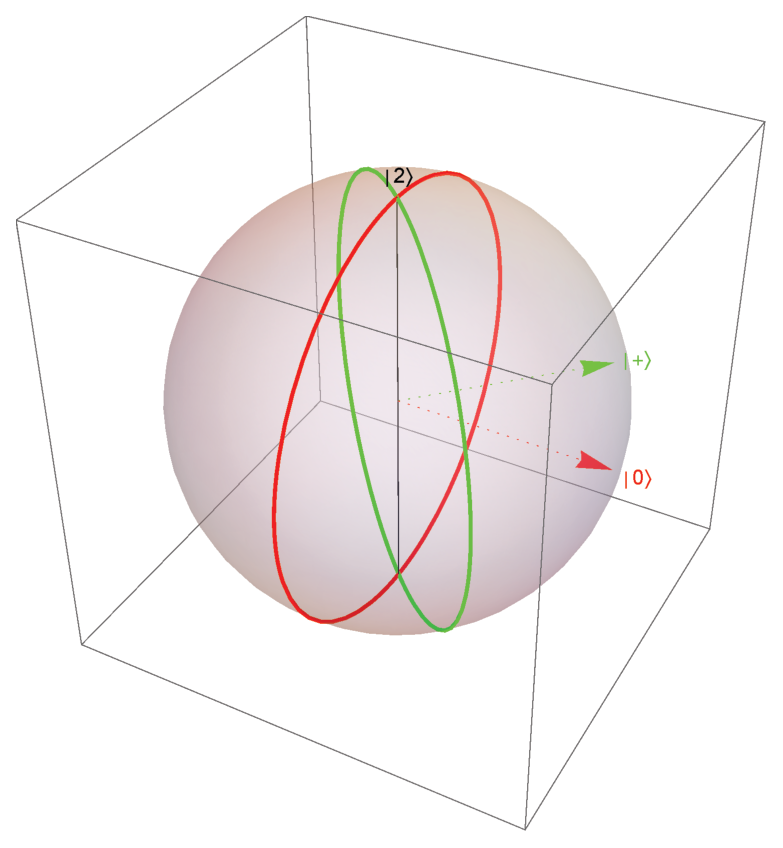
\includegraphics[scale=0.38]{figureE1} 
\par\end{centering}
\caption{\label{fig:three-dimensional-5-value}This figure illustrates cases
1 and 2 of example~\ref{ex:three-dimensional-5-value} plotted in
$\mathbb{R}^{3}$. The red and green dotted vectors are $\ket{0}$
and $\ket{\ps}$ respectively. All possible real vectors of the subspaces
orthogonal to $\ket{0}$ or $\ket{\ps}$ are drawn in the red and
green circles, respectively.}
\end{figure}

\begin{example}[Three-dimensional quantum 5-interval-valued probability
measure]\label{ex:three-dimensional-5-value} Given a three dimensional
Hilbert space with an orthonormal basis $\left\{ \ket{0},\ket{1},\ket{2}\right\} $.
Let\emph{ }$\ket{\ps}=\left(\ket{0}+\ket{1}\right)/\sqrt{2}$, and
$\mathscr{I}=\left\{ \imposs,\unlikely,\likely,\necess,\midd\right\} $,
where $\midd$ represents $\left[\frac{1}{4},\frac{3}{4}\right]$.
The definition of $\bar{\mu}$ below refers to figure~\ref{fig:three-dimensional-5-value}
which plots the 1-dimensional projectors: 
\begin{enumerate}
\item Let: 
\begin{equation}\eqalign{ 
\bar{\mu}(\mathbb{0})=\bar{\mu}(\proj{0})=\bar{\mu}(\proj{\ps})=\imposs\textrm{ ,}\\
\bar{\mu}(\mathbb{1})=\bar{\mu}(\mathbb{1}-\proj{0})=\bar{\mu}(\mathbb{1}-\proj{\ps})=\necess\textrm{ ,} 
}\end{equation}
where $\ket{0}$ and $\ket{\ps}$ are plotted as the red and green
dotted vectors, respectively. 
\item The red and green circles are the states orthogonal to $\ket{0}$
and $\ket{\ps}$, respectively. We define $\bar{\mu}\left(\proj{\psi}\right)=\bar{\mu}\left(\mathbb{1}-\proj{\psi}\right)=\midd$,
where $\ip{\psi}{0}=0$ or $\ip{\psi}{\ps}=0$.
\item Otherwise, $\bar{\mu}(\proj{\psi})=\unlikely$ and $\bar{\mu}(\mathbb{1}-\proj{\psi})=\likely$. 
\end{enumerate}
By theorem~\ref{thm:interval-valued-frame-function}, to check $\bar{\mu}$
a quantum interval-valued probability measure is equivalent to check
$\bar{f}$ satisfying 
\begin{equation}\eqalign{ 
\left[1,1\right]-\bar{f}\left(\ket{\psi_0}\right)\subseteq\bar{f}\left(\ket{\psi_1}\right)+\bar{f}\left(\ket{\psi_2}\right)\textrm{ ,}\\
\left[1,1\right]-\bar{f}\left(\ket{\psi_1}\right)\subseteq\bar{f}\left(\ket{\psi_2}\right)+\bar{f}\left(\ket{\psi_0}\right)\textrm{ ,}\\
\left[1,1\right]-\bar{f}\left(\ket{\psi_2}\right)\subseteq\bar{f}\left(\ket{\psi_0}\right)+\bar{f}\left(\ket{\psi_1}\right)
}\label{eq:non-additive-vectors}\end{equation}
for every orthonormal basis~$\left\{ \ket{\psi_{0}},\ket{\psi_{1}},\ket{\psi_{2}}\right\} $,
where $\bar{f}\left(\ket{\psi}\right)=\bar{\mu}\left(\proj{\psi}\right)$.
We are going to enumerate all possible orthonormal bases to verify
equation~(\ref{eq:non-additive-vectors}). Also, to simplify the
notation, we denote $\set{\ket{\psi}}{\ip{\psi}{0}\ne0\textrm{ and }\ip{\psi}{\ps}\ne0}$
by $\mathcal{T}$.
\begin{enumerate}
\item When $\ket{\psi_{0}}$ is $\ket{0}$, then $\ip{\psi_{1}}{0}=\ip{\psi_{2}}{0}=0$.
Equation~(\ref{eq:non-additive-vectors}) can then be verified as
follow. 
\begin{equation}\eqalign{ 
\left[1,1\right]-\bar{f}\left(\ket{0}\right)=\necess\subseteq\midd+\midd=\bar{f}\left(\ket{\psi_1}\right)+\bar{f}\left(\ket{\psi_2}\right)\textrm{ ,}\\
\left[1,1\right]-\bar{f}\left(\ket{\psi_1}\right)=\midd=\midd+\imposs=\bar{f}\left(\ket{\psi_2}\right)+\bar{f}\left(\ket{0}\right)\textrm{ ,}
}\end{equation}
Similarly, when $\ket{\psi_{0}}$ is $\ket{\ps}$, equation~(\ref{eq:non-additive-vectors})
holds. 
\item When $\ip{\psi_{0}}{0}=\ip{\psi_{1}}{\ps}=0$ and $\ket{\psi_{2}}\in\mathcal{T}$,
we have 
\begin{equation}\eqalign{ 
\left[1,1\right]-\bar{f}\left(\ket{\psi_0}\right)=\midd\subseteq\midd+\unlikely=\bar{f}\left(\ket{\psi_1}\right)+\bar{f}\left(\ket{\psi_2}\right)\textrm{ ,}\\
\left[1,1\right]-\bar{f}\left(\ket{\psi_2}\right)=\likely\subseteq\midd+\midd=\bar{f}\left(\ket{\psi_0}\right)+\bar{f}\left(\ket{\psi_1}\right)\textrm{ .}
}\end{equation}
\item When $\ip{\psi_{0}}{0}=0$, and $\ket{\psi_{1}}$, $\ket{\psi_{2}}\in\mathcal{T}$,
we have 
\begin{equation}\eqalign{ 
\left[1,1\right]-\bar{f}\left(\ket{\psi_0}\right)=\midd\subseteq\unlikely+\unlikely=\bar{f}\left(\ket{\psi_1}\right)+\bar{f}\left(\ket{\psi_2}\right)\textrm{ ,}\\
\left[1,1\right]-\bar{f}\left(\ket{\psi_1}\right)=\likely\subseteq\unlikely+\midd=\bar{f}\left(\ket{\psi_2}\right)+\bar{f}\left(\ket{\psi_0}\right)\textrm{ .}
}\end{equation}
Similarly, when $\ip{\psi_{0}}{\ps}=0$, $\ket{\psi_{1}}\in\mathcal{T}$,
and $\ket{\psi_{2}}\in\mathcal{T}$, equation~(\ref{eq:non-additive-vectors})
holds. 
\item When $\ket{\psi_{0}}$, $\ket{\psi_{1}}$, and $\ket{\psi_{2}}\in\mathcal{T}$,
i.e., the ``otherwise'' case. Then, equation~(\ref{eq:non-additive-vectors})
can easily be verified. 
\begin{equation}
\left[1,1\right]-\bar{f}\left(\ket{\psi_{0}}\right)=\likely\subseteq\unlikely+\unlikely=\bar{f}\left(\ket{\psi_{1}}\right)+\bar{f}\left(\ket{\psi_{2}}\right)\textrm{ .}
\end{equation}
\end{enumerate}
Since we proved that $\bar{\mu}$ is a quantum interval-valued probability
measure, $\bar{\mu}$ is convex by theorem~\ref{thm:convex-3}. 

The following argument establishes that $\bar{\mu}$ has an empty
core. Assume there is a real-valued probability measure satisfying
$\mu_{\rho}^{\mathrm{B}}(P)\in\bar{\mu}(P)$ for all $P\in\events$. Because
$\mu_{\rho}^{\mathrm{B}}(\proj{0})\in\bar{\mu}(\proj{0})=\imposs$ and $\mu_{\rho}^{\mathrm{B}}(\proj{\ps})\in\bar{\mu}(\proj{\ps})=\imposs$,
we must have $\mu_{\rho}^{\mathrm{B}}(\proj{0})=\mu_{\rho}^{\mathrm{B}}(\proj{\ps})=0$
so that $\mu_{\rho}^{\mathrm{B}}=\mu_{\ket{2}}^{\mathrm{B}}$. However, 
\begin{equation}
\mu_{\ket{2}}^{\mathrm{B}}(\proj{2})=1\notin\unlikely=\bar{\mu}(\proj{2})\textrm{ .}
\end{equation}
\end{example}

%%%%%%%%%%%%%%%%%%%%%%%%%%%%%%%%%%%%%%%%%%%%%%%%%%%%%%%%%%%%%%%%%%%%%%%%%%%%%%


\section{Contextuality and the Born Rule in Fuzzy Quantum Theories\label{sec:MerminSquare}}

\footnote{This section will be singled out as a separated letter.}The
Kochen-Specker theorem asserts that there is no function~$v$ assigning
a definitely value to all observables such that
\begin{equation}\eqalign{ 
v\left(O_{1}\right)+v\left(O_{2}\right)=v\left(O_{1}+O_{2}\right)\textrm{ and}\\
v\left(O_{1}\right)v\left(O_{2}\right)=v\left(O_{1}O_{2}\right)
}\label{eq:Kochen-Specker-Rules}\end{equation}
if $O_{1}$ and $O_{2}$ are commuting observables. Suppose that there
is a function~$v$ satisfying these two properties, it must send
an observable to its eigenvalues so that the following observables~\cite{Mermin1990Simple,peres1995quantum}:
\begin{equation}
\begin{array}{ccc}
\mathbb{1}\otimes\sigma_{z} & \sigma_{z}\otimes\mathbb{1} & \sigma_{z}\otimes\sigma_{z}\\
\sigma_{x}\otimes\mathbb{1} & \mathbb{1}\otimes\sigma_{x} & \sigma_{x}\otimes\sigma_{x}\\
\sigma_{x}\otimes\sigma_{z} & \sigma_{z}\otimes\sigma_{x} & \sigma_{y}\otimes\sigma_{y}
\end{array}\label{eq:MerminSquare}
\end{equation}
must be sent to $1$ or $-1$. In each row and column, operators commutes,
and each operator is the product of the two others, except in the
third column $\left(\sigma_{z}\otimes\sigma_{z}\right)\left(\sigma_{x}\otimes\sigma_{x}\right)=-\sigma_{y}\otimes\sigma_{y}$.
Therefore, it is clear impossible to find a function~$v$ such that
\begin{equation}
\begin{array}{ccc}
v\left(\mathbb{1}\otimes\sigma_{z}\right) & v\left(\sigma_{z}\otimes\mathbb{1}\right) & v\left(\sigma_{z}\otimes\sigma_{z}\right)\\
v\left(\sigma_{x}\otimes\mathbb{1}\right) & v\left(\mathbb{1}\otimes\sigma_{x}\right) & v\left(\sigma_{x}\otimes\sigma_{x}\right)\\
v\left(\sigma_{x}\otimes\sigma_{z}\right) & v\left(\sigma_{z}\otimes\sigma_{x}\right) & v\left(\sigma_{y}\otimes\sigma_{y}\right)
\end{array}\label{eq:MerminSquare-values}
\end{equation}
satisfying equation~(\ref{eq:Kochen-Specker-Rules}).

\begin{table}
\caption{\label{table:commonBasis}In each row, three observables are listed
in the left column commutes, and their common eigenbasis is listed
in the right column. In order to unified and simplify notation, we
do not normalize eigenstates, and represent the state~$\alpha_{0}\ket{0}+\alpha_{1}\ket{1}+\alpha_{2}\ket{2}+\alpha_{3}\ket{3}$
as $\left(\alpha_{0},\alpha_{1},\alpha_{2},\alpha_{3}\right)$.}

\begin{tabular}{ccc|cccc} 
\br 
\multicolumn{3}{c}{Commuting observables} & \multicolumn{4}{c}{Common eigenbasis} \\
\mr 
$\mathbb{1}\otimes\sigma_{z}$ & $\sigma_{z}\otimes\mathbb{1}$ & $\sigma_{z}\otimes\sigma_{z}$ & $(1, 0, 0, 0)$ & $(0, 1, 0, 0)$ & $(0, 0, 1, 0)$ & $(0, 0, 0, 1)$ \\
$\sigma_{x}\otimes\mathbb{1}$ & $\mathbb{1}\otimes\sigma_{x}$ & $\sigma_{x}\otimes\sigma_{x}$ & $(1, 1, 1, 1)$ & $(1, -1, 1, -1)$ & $(1, 1, -1, -1)$ & $(1, -1, -1, 1)$ \\
$\sigma_{x}\otimes\sigma_{z}$ & $\sigma_{z}\otimes\sigma_{x}$ & $\sigma_{y}\otimes\sigma_{y}$ & $(1, 1, 1, -1)$ & $(1, 1, -1, 1)$ & $(1, -1, 1, 1)$ & $(-1, 1, 1, 1)$ \\
$\mathbb{1}\otimes\sigma_{z}$ & $\sigma_{x}\otimes\mathbb{1}$ & $\sigma_{x}\otimes\sigma_{z}$ & $(1, 0, 1, 0)$ & $(0, 1, 0, 1)$ & $(1, 0, -1, 0)$ & $(0, 1, 0, -1)$ \\
$\sigma_{z}\otimes\mathbb{1}$ & $\mathbb{1}\otimes\sigma_{x}$ & $\sigma_{z}\otimes\sigma_{x}$ & $(1, 1, 0, 0)$ & $(1, -1, 0, 0)$ & $(0, 0, 1, 1)$ & $(0, 0, 1, -1)$ \\
$\sigma_{z}\otimes\sigma_{z}$ & $\sigma_{x}\otimes\sigma_{x}$ & $\sigma_{y}\otimes\sigma_{y}$ & $(0, 1, 1, 0)$ & $(0, 1, -1, 0)$ & $(1, 0, 0, 1)$ & $(1, 0, 0, -1)$ \\
\br 
\end{tabular} 
\end{table}
Since observables in equation~(\ref{eq:MerminSquare}) are not projections,
if we want to reformulate the above argument in the language of quantum
probability measures, we first need to find the common eigenbasis
of each row and column, and consider the projections to each eigenvectors.
Let $\mathcal{T}_{24}$ denote all eigenstates listed in table~\ref{table:commonBasis}.
The Kochen-Specker theorem could then be proved by showing there is
no function~$v:\events_{24}\rightarrow\left\{ 0,1\right\} $ satisfying
equation~(\ref{eq:Kochen-Specker-Rules}), where 
\begin{equation}
\events_{24}=\set{\sum_{i=1}^{N}\proj{\psi_{i}}}{\textrm{mutually orthogonal }\left\{ \ket{\psi_{i}}\right\} _{i=1}^{N}\subseteq\mathcal{T}_{24}}
\end{equation}
which is a sub-event space defined in definition~\ref{def:sub-event-space}.
This kind of $v$ is actually a quantum cryptodeterministic measure.
Since a cryptodeterministic measure is a special case of real-valued
probability measure, by theorem~\ref{lemma:classical-probability-measures},
the quantum cryptodeterministic measure~$v$ exists if and only if
there exists a frame function~$f:\mathcal{T}_{24}\rightarrow\left\{ 0,1\right\} $
which should at least satisfy
\begin{equation}\eqalign{ 
1 = f(1, 0, 0, 0) + f(0, 1, 0, 0) + f(0, 0, 1, 0) + f(0, 0, 0, 1)\textrm{ and}\\
1 = f(-1, 1, 1, 1) + f(1, -1, 1, 1) + f(1, 1, -1, 1) + f(1, 1, 1, -1)
}\label{eq:Kernaghan-1}\end{equation}
because of table~\ref{table:commonBasis}. $f$ should also satisfy
the following equations since the vectors in each equation form an
orthogonal basis~\cite{Kernaghan1994,peres1995quantum}:
\begin{equation}\eqalign{ 
1 = f(1, 0, 0, 0) + f(0, 1, 0, 0) + f(0, 0, 1, 1) + f(0, 0, 1, -1)\textrm{ ,}\\
1 = f(1, 0, 0, 0) + f(0, 0, 1, 0) + f(0, 1, 0, 1) + f(0, 1, 0, -1)\textrm{ ,}\\
1 = f(1, 0, 0, 0) + f(0, 0, 0, 1) + f(0, 1, 1, 0) + f(0, 1, -1, 0)\textrm{ ,}\\
1 = f(-1, 1, 1, 1) + f(1, 1, -1, 1) + f(1, 0, 1, 0) + f(0, 1, 0, -1)\textrm{ ,}\\
1 = f(-1, 1, 1, 1) + f(1, 1, -1, 1) + f(0, 1, 1, 0) + f(1, 0, 0, -1)\textrm{ ,}\\
1 = f(1, 1, -1, 1) + f(1, 1, 1, -1) + f(0, 0, 1, 1) + f(1, -1, 0, 0)\textrm{ ,}\\
1 = f(0, 1, -1, 0) + f(1, 0, 0, -1) + f(1, 1, 1, 1) + f(1, -1, -1, 1)\textrm{ ,}\\
1 = f(0, 0, 1, -1) + f(1, -1, 0, 0) + f(1, 1, 1, 1) + f(1, 1, -1, -1)\textrm{ ,}\\
1 = f(1, 0, 1, 0) + f(0, 1, 0, 1) + f(1, 1, -1, -1) + f(1, -1, -1, 1)\textrm{ .}
}\label{eq:Kernaghan-2}\end{equation}
In equation~\ref{eq:Kernaghan-1} and \ref{eq:Kernaghan-2}, there
are odd number of equations, but each $f\left(\alpha_{0},\alpha_{1},\alpha_{2},\alpha_{3}\right)$
occurs twice. Therefore, there is no frame function~$f:\mathcal{T}_{24}\rightarrow\left\{ 0,1\right\} $
satisfying equation~\ref{eq:Kernaghan-1} and \ref{eq:Kernaghan-2}.

On one hand, the Kochen-Specker theorem is equivalent to non-existence
of quantum cryptodeterministic measure~$\mu^{\mathrm{D}}:\events\rightarrow\left\{ 0,1\right\} $,
where $\events$ is the set of all projections on a Hilbert space.
On the other hand, if we replace the range by the interval~$\left[0,1\right]$,
Gleason's theorem asserts that every quantum real-valued probability
measure~$\mu:\events\rightarrow\left[0,1\right]$ can be induced
by a density matrix according to the Born rule. These two extreme
cases can be understood in a broader framework of quantum interval-valued
probability measure (IVPM)~$\bar{\mu}:\events\rightarrow\mathscr{I}$,
where $\mathscr{I}$ is a collection of intervals containing in $\left[0,1\right]$.
When we pick $\mathscr{I}$ as $\mathscr{I}_{\mathrm{D}}=\left\{ \imposs,\necess\right\} $,
where $\imposs=\left[0,0\right]$ and $\necess=\left[1,1\right]$,
there is no quantum IVPM~$\bar{\mu}:\events\rightarrow\mathscr{I}$
by corollary~\ref{cor:Kochen-Specker-IVPM} of the Kochen-Specker
theorem. When the collection of intervals is $\mathscr{I}_{\infty}=\set{\left[x,x\right]}{x\in\left[0,1\right]}$,
a quantum IVPM is well-behaved as a usual quantum real-valued probability
measure does. 

Given any sub-event space~$\events'\subseteq\events$, in order to
qualify how well-behaved a quantum IVPM~$\bar{\mu}:\events'\rightarrow\mathscr{I}$
could be, we introduce the notion of core.

\begin{definition}A \emph{core} of $\bar{\mu}$ is the set $\mathrm{core}\left(\bar{\mu}\right)=\set{\pmeas:\events'\rightarrow[0,1]}{\forall P\in\events'.~\pmeas\left(P\right)\in\bar{\mu}\left(P\right)}$.\end{definition}

\noindent Then, Gleason's theorem guarantees that $\bar{\mu}$ has
a unique core element for any $\bar{\mu}:\events\rightarrow\mathscr{I}_{\infty}$.
In the rest of the letter, we will provide examples of quantum IVPMs
on $\events_{24}$, and show how a quantum IVPM~$\bar{\mu}:\events_{24}\rightarrow\mathscr{I}$
could be depending on different intervals~$\mathscr{I}$.

First, based on a Born rule probability measure, say $\mu_{\ket{0}}^{\mathrm{\mathrm{B}}}$,
it is easy to construct a quantum IVPM~$\bar{\mu}:\events_{24}\rightarrow\mathscr{I}$
whose unique core element is $\mu_{\ket{0}}^{\mathrm{\mathrm{B}}}$.
For example, when $\mathscr{I}$ is $\left\{ \imposs,\necess,\left[\frac{1}{4},\frac{1}{4}\right],\left[\frac{1}{2},\frac{1}{2}\right],\left[\frac{3}{4},\frac{3}{4}\right]\right\} $,
we have $\iota_{\infty}\circ\mu_{\ket{0}}^{\mathrm{\mathrm{B}}}:\events_{24}\rightarrow\mathscr{I}$
and $\mathrm{core}\left(\iota_{\infty}\circ\mu_{\ket{0}}^{\mathrm{\mathrm{B}}}\right)=\left\{ \mu_{\ket{0}}^{\mathrm{\mathrm{B}}}\right\} $,
where $\iota_{\infty}\left(x\right)=\left[x,x\right]$ and $\circ$
denote function composition. This provides an example that a well-behaved
quantum IVPM exists even if $\mathscr{I}$ is discrete. Well-behaved
quantum IVPMs happen when mapping to other kind of intervals. For
example, we can add an one extra interval~$\unknown=\left[0,1\right]$
to $\mathscr{I}_{\mathrm{D}}$, and consider $\mathscr{I}_{1}=\left\{ \imposs,\unknown,\necess\right\} $.
Let 
\begin{equation} 
\iota_1(x)=\cases{ 
\necess & if $x=1$ ;\\ 
\imposs & if $x=0$ ;\\ 
\unknown & otherwise. 
}\label{eq:homomorphism-1} \end{equation}
, and we still have $\mathrm{core}\left(\iota_{1}\circ\mu_{\ket{0}}^{\mathrm{\mathrm{B}}}\right)=\left\{ \mu_{\ket{0}}^{\mathrm{\mathrm{B}}}\right\} $.

\footnote{\yutsung{Find all orthogonal basis of $\mathcal{T}_{24}$ and solve
the linear equations for Gleason's...}}

%%%%%%%%%%%%%%%%%%%%%%%%%%%%%%%%%%%%%%%%%%%%%%%%%%%%%%%%%%%%%%%%%%%%%%%%%%%%%%
\begin{comment}
 \bibliographystyle{plain}
\bibliography{prop}
 
\end{comment}
\printbibliography

\end{document}

%%%%%%%%%%%%%%%%%%%%%%%%%%%%%%%%%%%%%%%%%%%%%%%%%%%%%%%%%%%%%%%%%%%%%%%%%%%%%%



